%\begin{center}
%\includegraphics[scale=0.05, angle=-90]{figboga/remark.JPG}
%\end{center}
\documentclass{article}
\usepackage[utf8]{inputenc}
\usepackage{amsmath}
\usepackage{xcolor}
\newcommand{\red}[1]{\textcolor{red}{#1}}
\usepackage{hyperref}
\usepackage{amsfonts}
\usepackage{listings}
\usepackage{color}
\definecolor{dkgreen}{rgb}{0,0.6,0}
\definecolor{gray}{rgb}{0.5,0.5,0.5}
\definecolor{mauve}{rgb}{0.58,0,0.82}
\lstset{frame=tb,
  language=Python,
  aboveskip=3mm,
  escapechar=\%,
  belowskip=3mm,
  showstringspaces=false,
  columns=flexible,
  basicstyle={\small\ttfamily},
  numbers=none,
  numberstyle=\tiny\color{black},
  keywordstyle=\color{black},
  commentstyle=\color{dkgreen},
  stringstyle=\color{black},
  breaklines=true,
  breakatwhitespace=true,
  tabsize=3
}
\usepackage{ mathrsfs }
\usepackage{amsthm}
\usepackage{amssymb}
\usepackage{graphics}
\usepackage{graphicx}
\usepackage{mathtools}
\usepackage{booktabs}
\DeclareMathOperator\dom{dom}
\DeclareMathOperator\vphi{\varphi}
\DeclareMathOperator\eps{\epsilon}
\DeclareMathOperator\del{\delta}
\DeclareMathOperator\Del{\Delta}
\DeclareMathOperator\lm{\lambda}
\DeclareMathOperator\deq{\vcentcolon=}
\DeclareMathOperator\R{\mathbb{R}}
\DeclareMathOperator\pr{\mathbb{P}}
\DeclareMathOperator\Z{\mathbb{Z}}
\DeclareMathOperator\N{\mathbb{N}}
\DeclareMathOperator\F{\mathbb{F}}
\DeclareMathOperator\A{\mathbb{A}}
\DeclareMathOperator\HH{\mathbb{H}}
\DeclareMathOperator\minn{\text{Minimise} \quad }
\DeclareMathOperator\maxx{\text{Maximise} \quad }
\DeclareMathOperator\st{\text{Subject to} \quad }
\DeclareMathOperator\nc{\text{no constraints}}
\DeclarePairedDelimiter\ceil{\lceil}{\rceil}
\DeclarePairedDelimiter\floor{\lfloor}{\rfloor}
\DeclareMathOperator\bx{\bold{x}}
\DeclareMathOperator\bs{\bold{s}}
\DeclareMathOperator\id{\text{Id}}
\DeclareMathOperator\bb{\bold{b}}
\DeclareMathOperator\bA{\bold{A}}
\DeclareMathOperator\bp{\bold{p}}
\DeclareMathOperator\bc{\bold{c}}
\DeclareMathOperator\C{\mathbb{C}}
\DeclareMathOperator\ran{ran}
\DeclareMathOperator\img{Im}
\DeclareMathOperator\op{\oplus}
\DeclareMathOperator\ot{\otimes}
\DeclareMathOperator\diam{diam}
\DeclareMathOperator\ite{int}
\DeclareMathOperator*{\argmax}{arg\,max}
\DeclareMathOperator*{\argmin}{arg\,min}
\DeclareMathOperator\cd{card}
\DeclareMathOperator\la{\langle}
\DeclareMathOperator\ra{\rangle}
\DeclareMathOperator\erf{erf}
\DeclareMathOperator\erfc{erfc}
\DeclareMathOperator\iso{\,\simeq\,}
\DeclareMathOperator{\sgn}{sgn}
\DeclareMathOperator{\lcm}{lcm}

\newcommand{\an}[1]{\langle \, #1 \, \rangle}
\newcommand{\GL}{\text{GL}(\mathbb{R}^n)}
\newcommand{\GLM}{\text{GL}(n,\mathbb{R})}
\newcommand{\quo}{/ _\sim}
\newcommand{\phii}{\phi^{-1}}
\newcommand{\pa}{\partial}
\newcommand{\lb}{\left}
\newcommand{\rb}{\right}
\newcommand{\aps}{\alpha_S}
\newcommand{\apl}{\alpha_L}
\newcommand{\tdd}{\frac{d^2T}{dx^2}}
\newcommand{\dx}{\frac{d}{dx}}
\newcommand{\seq}{(x_n)_{n \geq 1}}
\newcommand{\sseq}{(x_{n_k})_{k \geq 1}}
\newcommand{\fseq}{(f_n)_{n \geq 1}}
\newcommand{\elll}{\ell^{\infty}(\N)}
\newcommand{\norm}{{\|.\|}}
\newcommand{\inner}{\langle .,. \rangle}
\newcommand*\dd{\, \mathop{}\!\mathrm{d}}
\newcommand*\DD[1]{\, \mathop{}\!\mathrm{d^#1}}
\newcommand{\Ga}[1]{\frac{1}{\sqrt{2\pi\sigma^2}} e^{-\frac{\left(#1\right)^2}{2\sigma^2}}}
\usepackage{color}
%\title{}
\newcommand*\autoop{\left(}
\newcommand*\autocp{\right)}
\newcommand*\autoob{\left[}
\newcommand*\autocb{\right]}
\DeclareRobustCommand*\{{\ifmmode \left\lbrace \else \textbraceleft \fi }
\DeclareRobustCommand*\}{\ifmmode \right\rbrace \else \textbraceright \fi }
\AtBeginDocument {%
   \mathcode`( 32768
   \mathcode`) 32768
   \mathcode`[ 32768
   \mathcode`] 32768
   \begingroup
       \lccode`\~`(
       \lowercase{%
   \endgroup
       \let~\autoop
   }\begingroup
       \lccode`\~`)
       \lowercase{%
   \endgroup
       \let~\autocp
   }\begingroup
       \lccode`\~`[
       \lowercase{%
   \endgroup
       \let~\autoob
   }\begingroup
       \lccode`\~`]
       \lowercase{%
   \endgroup
       \let~\autocb
   }}

\delimiterfactor 1001

\makeatletter
% for amsmath "compatibility" (not sophisticated)
% \usepackage{amsmath}
\AtBeginDocument {%
          \def\resetMathstrut@{%
           \setbox\z@\hbox{\the\textfont\symoperators\char40}%
           \ht\Mathstrutbox@\ht\z@ \dp\Mathstrutbox@\dp\z@}%
}%
\makeatother
\author{Brendan Matthews}
\title{I forget}
\begin{document}
\maketitle{}
\newpage{}
\section*{Chapter -1}
Group tables are dumb and playing sudoku doesn't guarantee associativity.
\begin{center}
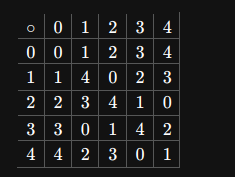
\includegraphics[scale=0.6, angle=-0]{fig/countergroup.png}
\end{center}
$D_3 = S_3$ but $D_n \neq S_n, \quad n \geq 4$.
\begin{center}
\includegraphics[scale=0.6, angle=-90]{fig/IMG_7240.jpeg}
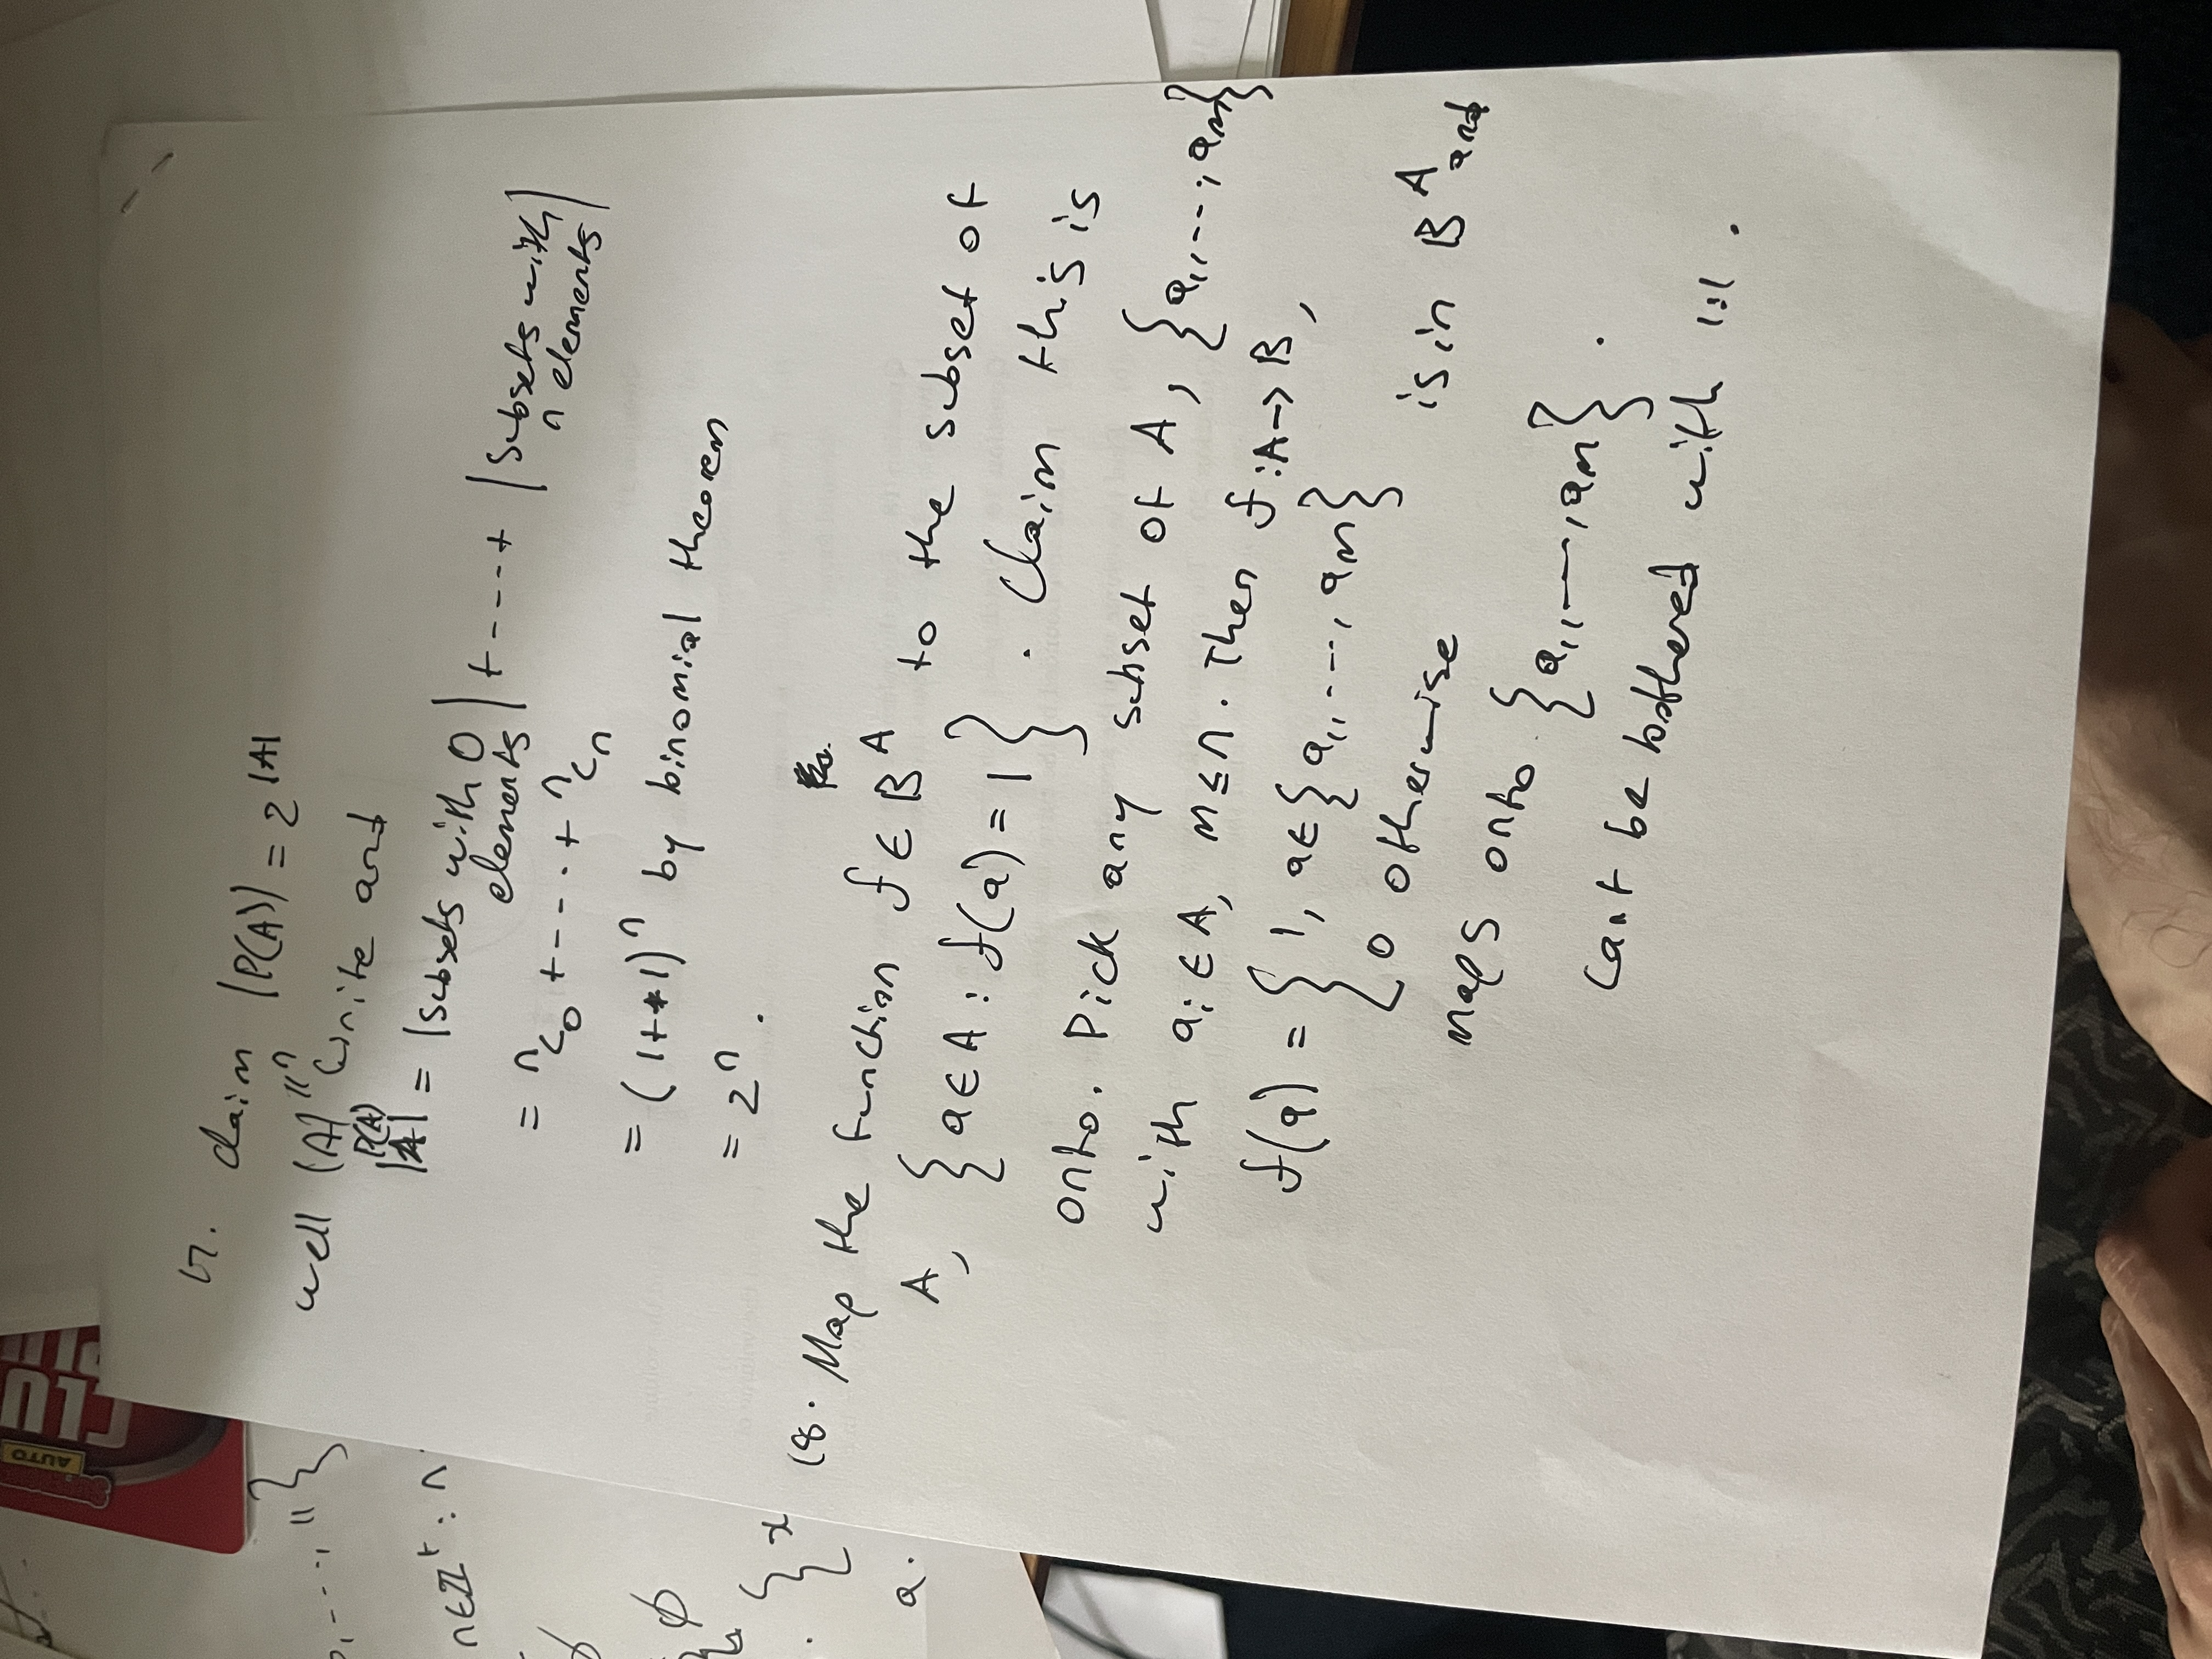
\includegraphics[scale=0.6, angle=-90]{fig/IMG_7241.jpeg}
\end{center}
\section{}
A binary operation is a map $*:S \times S \to S$ and a subset $H$ of $S$ is closed under $*$ if the obvious thing happens.
We say that $*$ is induced on $H$. There are $n^{n^2}$ binary ops on a set of size $n$ and $n^{\sum_n i} = n^{\frac{n(n+1)}{2}}$ commutative ones.
The latter is because the number of elements of $S \times S$ that aren't predetermined by the condition is $n+(n-1)+\hdots+1$ and schoolboy Gauss does the rest.
Note that for finite $A,B$, number of maps from $A$ to $B$ is $|B|^{|A|}$.
\begin{center}
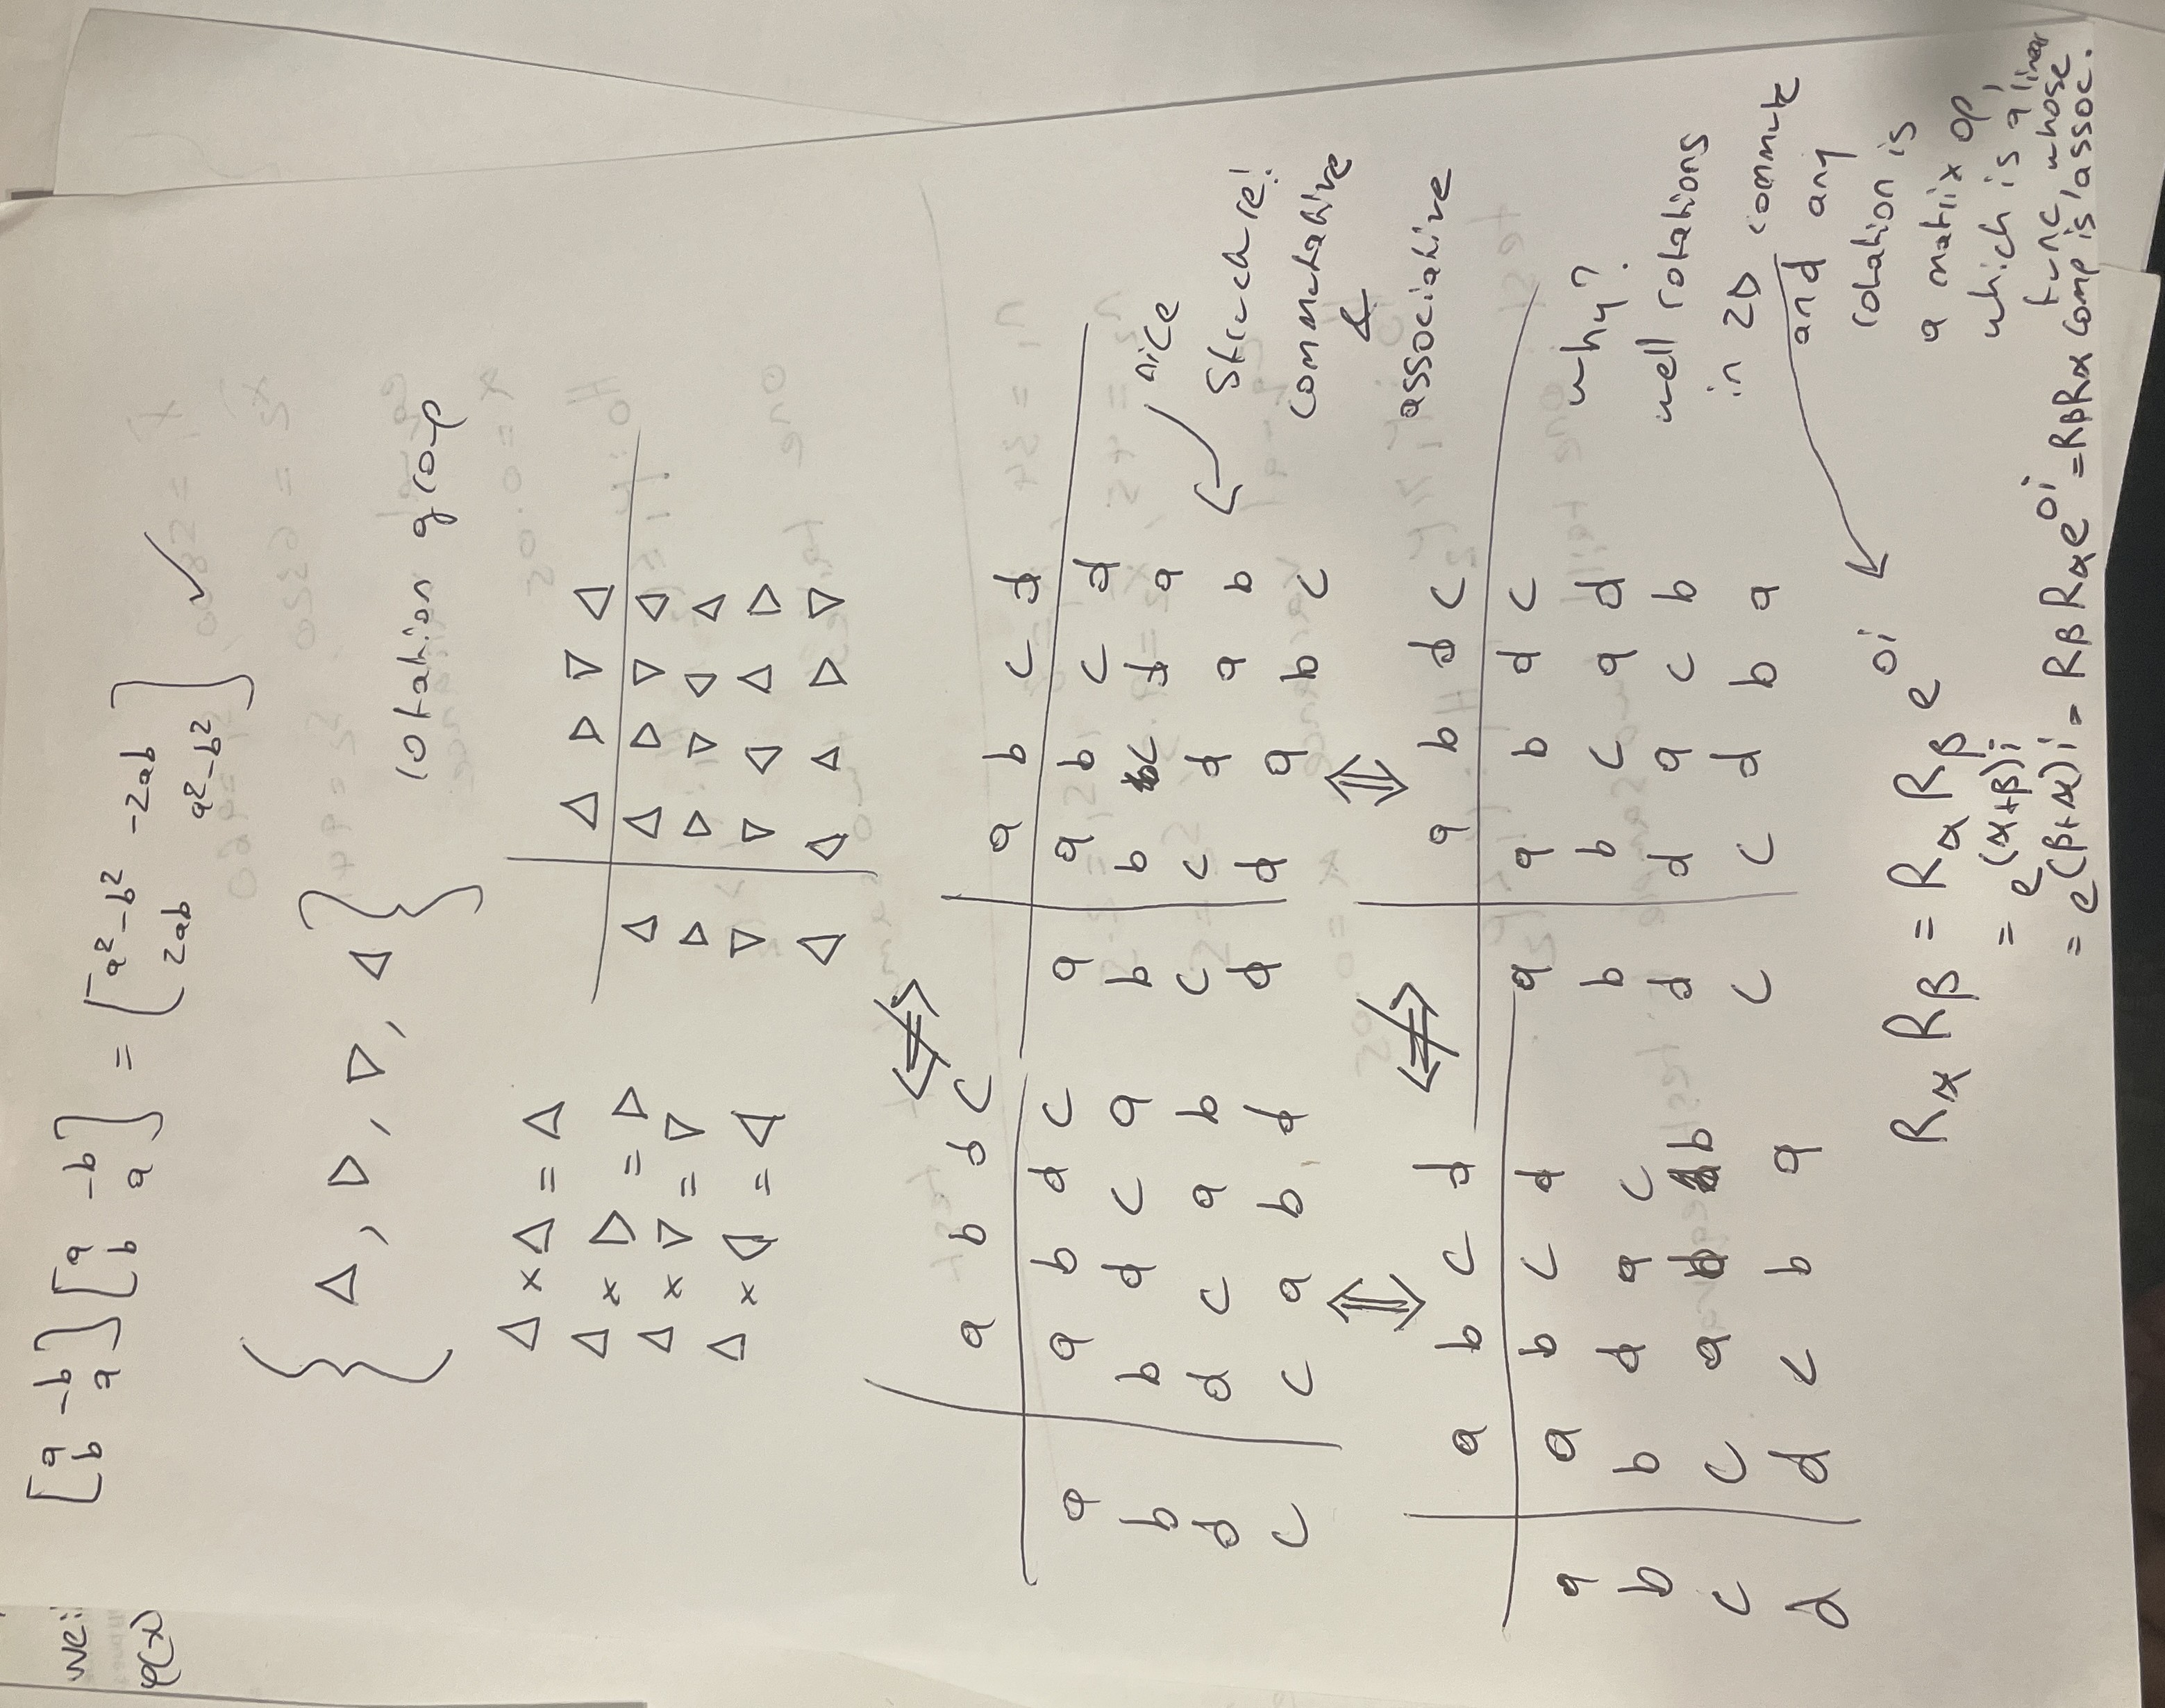
\includegraphics[scale=0.1, angle=-90]{fig/IMG_7243.jpeg}
\end{center}
Not every 2 element commuter is associative. Consider $aa = b, \,\, ab=b,\,\,ba=b,\,\,bb=a$ and $a(ab) = ab=b,\,\,(aa)b=bb=a$. 35 is rubbish.
\begin{center}
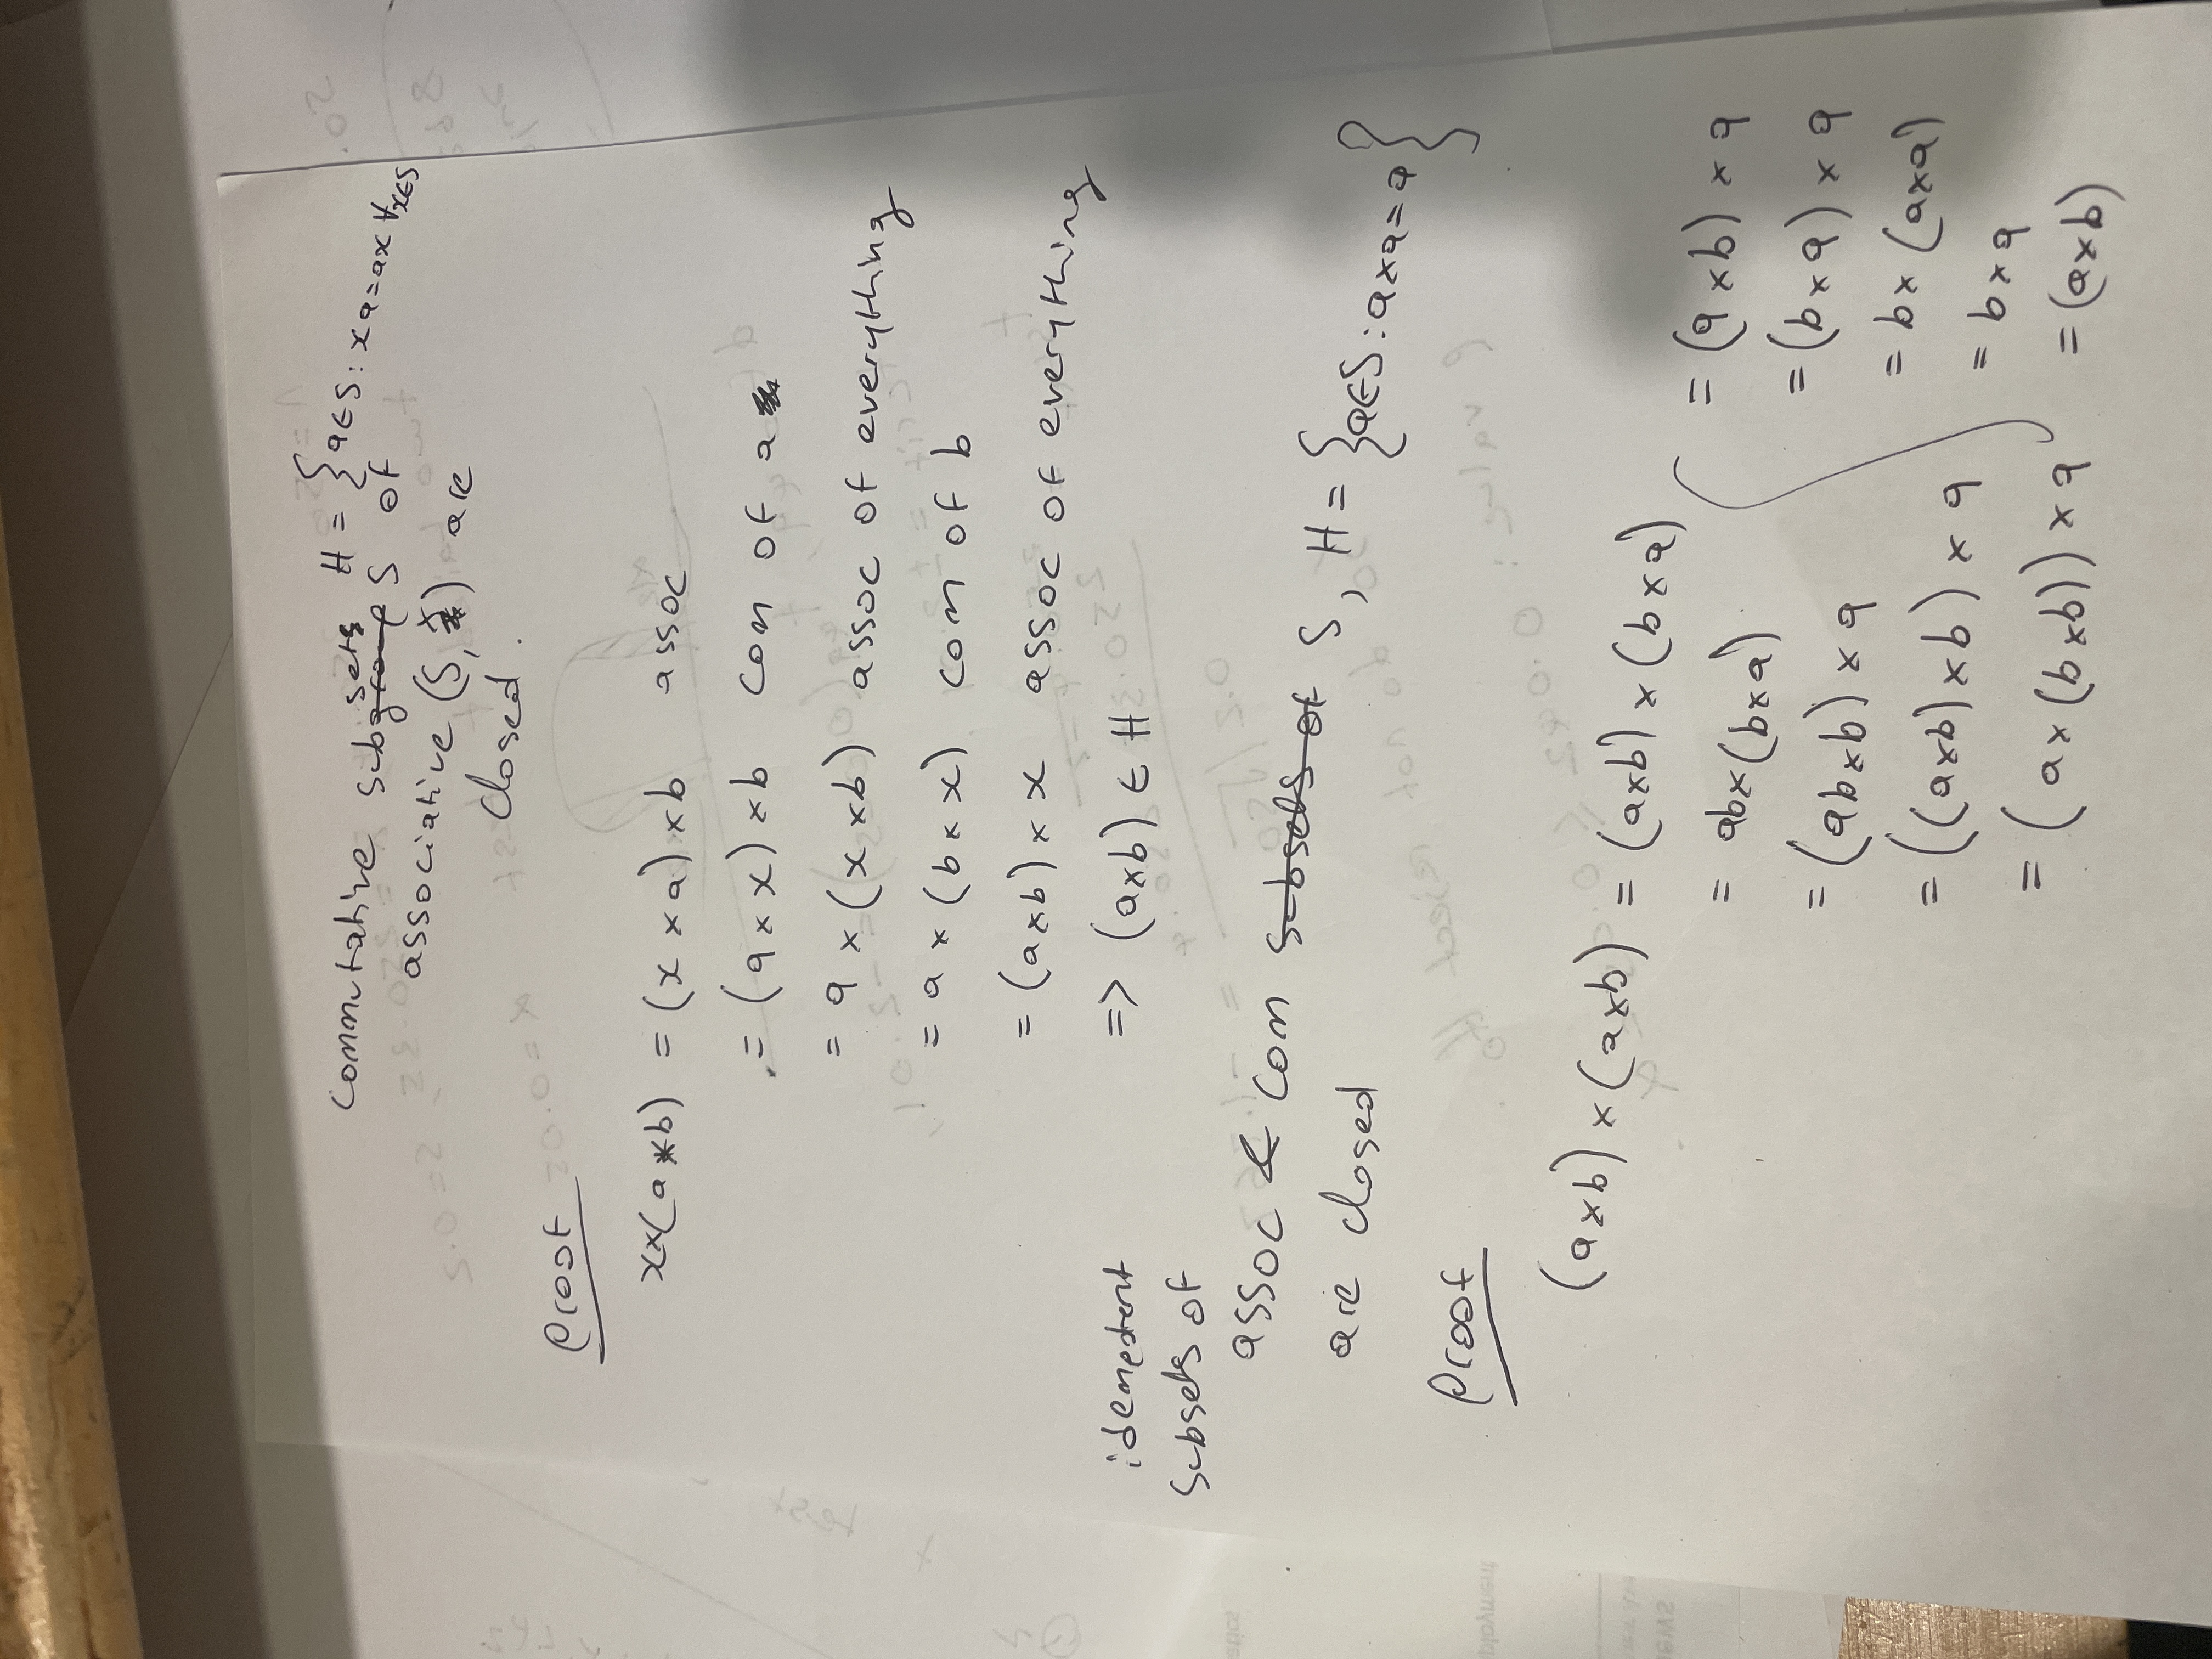
\includegraphics[scale=0.4, angle=-90]{fig/IMG_7244.jpeg}
\end{center}
\section*{}
Two binary algebraic structures $(R,*),(S,+)$ are isomorphic, $R \iso S$, if for each $x,y \in R$ with $x*y = z$,
we have corresponding $x',y',z' \in S$ so that $x' + y' = z'$. That is,
there exists a bijection $\phi:R \to S$ such that for all $x,y \in R$ with $x*y=z$,
\[
\phi(x*y) = \phi(x)+\phi(y) = x'+y' = z' = \phi(z).
\]
Each point in $S$ is mapped to by exactly one point in $R$. Isomorphism is an equivalence relation.
\begin{proof}
$S \iso S$ by identity map. If $R \iso S$, then there exists $\phi:R \to S$, bijective and a homomorphism. So the inverse exists.
The inverse is a homomorphism by injectivity of $\phi$: $$
\phi(\phii(s_1)*\phii(s_2)) \underset{\text{H prop of $\phi$}}{=} \phi(\phii(s_1))+\phi(\phii(s_2)) = s_1 + s_2 = \phi(\phii(s_1+s_2)).
$$
Transitivity is easy just compose the isos.
\end{proof}
\subsection*{Theorem}
Suppose there is an onto homomorphism $\phi:(R,+) \to (S,*)$ and an identity $e \in R$. Then $\phi(e) \in S$ is an identity.
\begin{proof}
Easy.
\end{proof}
Note that while the identity is always unique in $S$, we require that $\phi$ be an isomorphism for the preimage of the identity to be uniquely the identity of $R$.
\subsection*{Theorem}
Suppose $S$ is a \textbf{group} and $R,S$ have identities $e_R,e_S$. If there is a homomorphism $\phi:(R,+) \to (S,*)$, then $\phi(e_R) = e_S$.
\begin{proof}
$$
\phi(e_R) = \phi(e_R+e_R) = \phi(e_R) * \phi(e_R)
$$
Apply inverse of $\phi(e_R)$.
\end{proof}
\subsection*{Non Isomorphism Example}
The function $\phi: (M_2(\R),\times) \to (\R,\times), \quad \phi(A) = \det(A)$ is not an isomorphism (in fact, no such isomorphism exists).
\begin{proof}
It is a homomorphism, $\det(AB) = \det(A)\det(B)$. But it isn't injective because matrix multiplication isn't commutative.
Take $$A = \begin{bmatrix}
1 & 1 \\
0 & 1
\end{bmatrix},\quad B =
\begin{bmatrix}
1 & 0 \\
1 & 1
\end{bmatrix}
$$
then $$
AB = \begin{bmatrix}
2 & 1 \\
1 & 1
\end{bmatrix},\quad BA =
\begin{bmatrix}
1 & 1 \\
1 & 2
\end{bmatrix}
$$
so that $$
\phi(AB) = \phi(BA) = 1 \text{ but } AB \neq BA.
$$
\end{proof}
\noindent Another example that fails injectivity is the map under addition from functions with derivatives to their derivatives.
Being a binary operation (or even a function at all) can fail with integrals even if everything else works.
\subsection*{Disproof using stuff that's preserved under isomorphisms}
We know the identity is preserved. So $\phi(f)(x) = xf(x)$ is not an isomorphism across $F = \{f: \R \to \R| f \text{ is smooth}\}$ under multiplication, $\phi(\bf{1})(2) = 2 \neq 1$, so $\phi(\bf{1}) \neq \bf{1}$, where $\bf{1}: \R \to \R$ is given by $\bf{1}$$ (x) = 1$.
\begin{center}
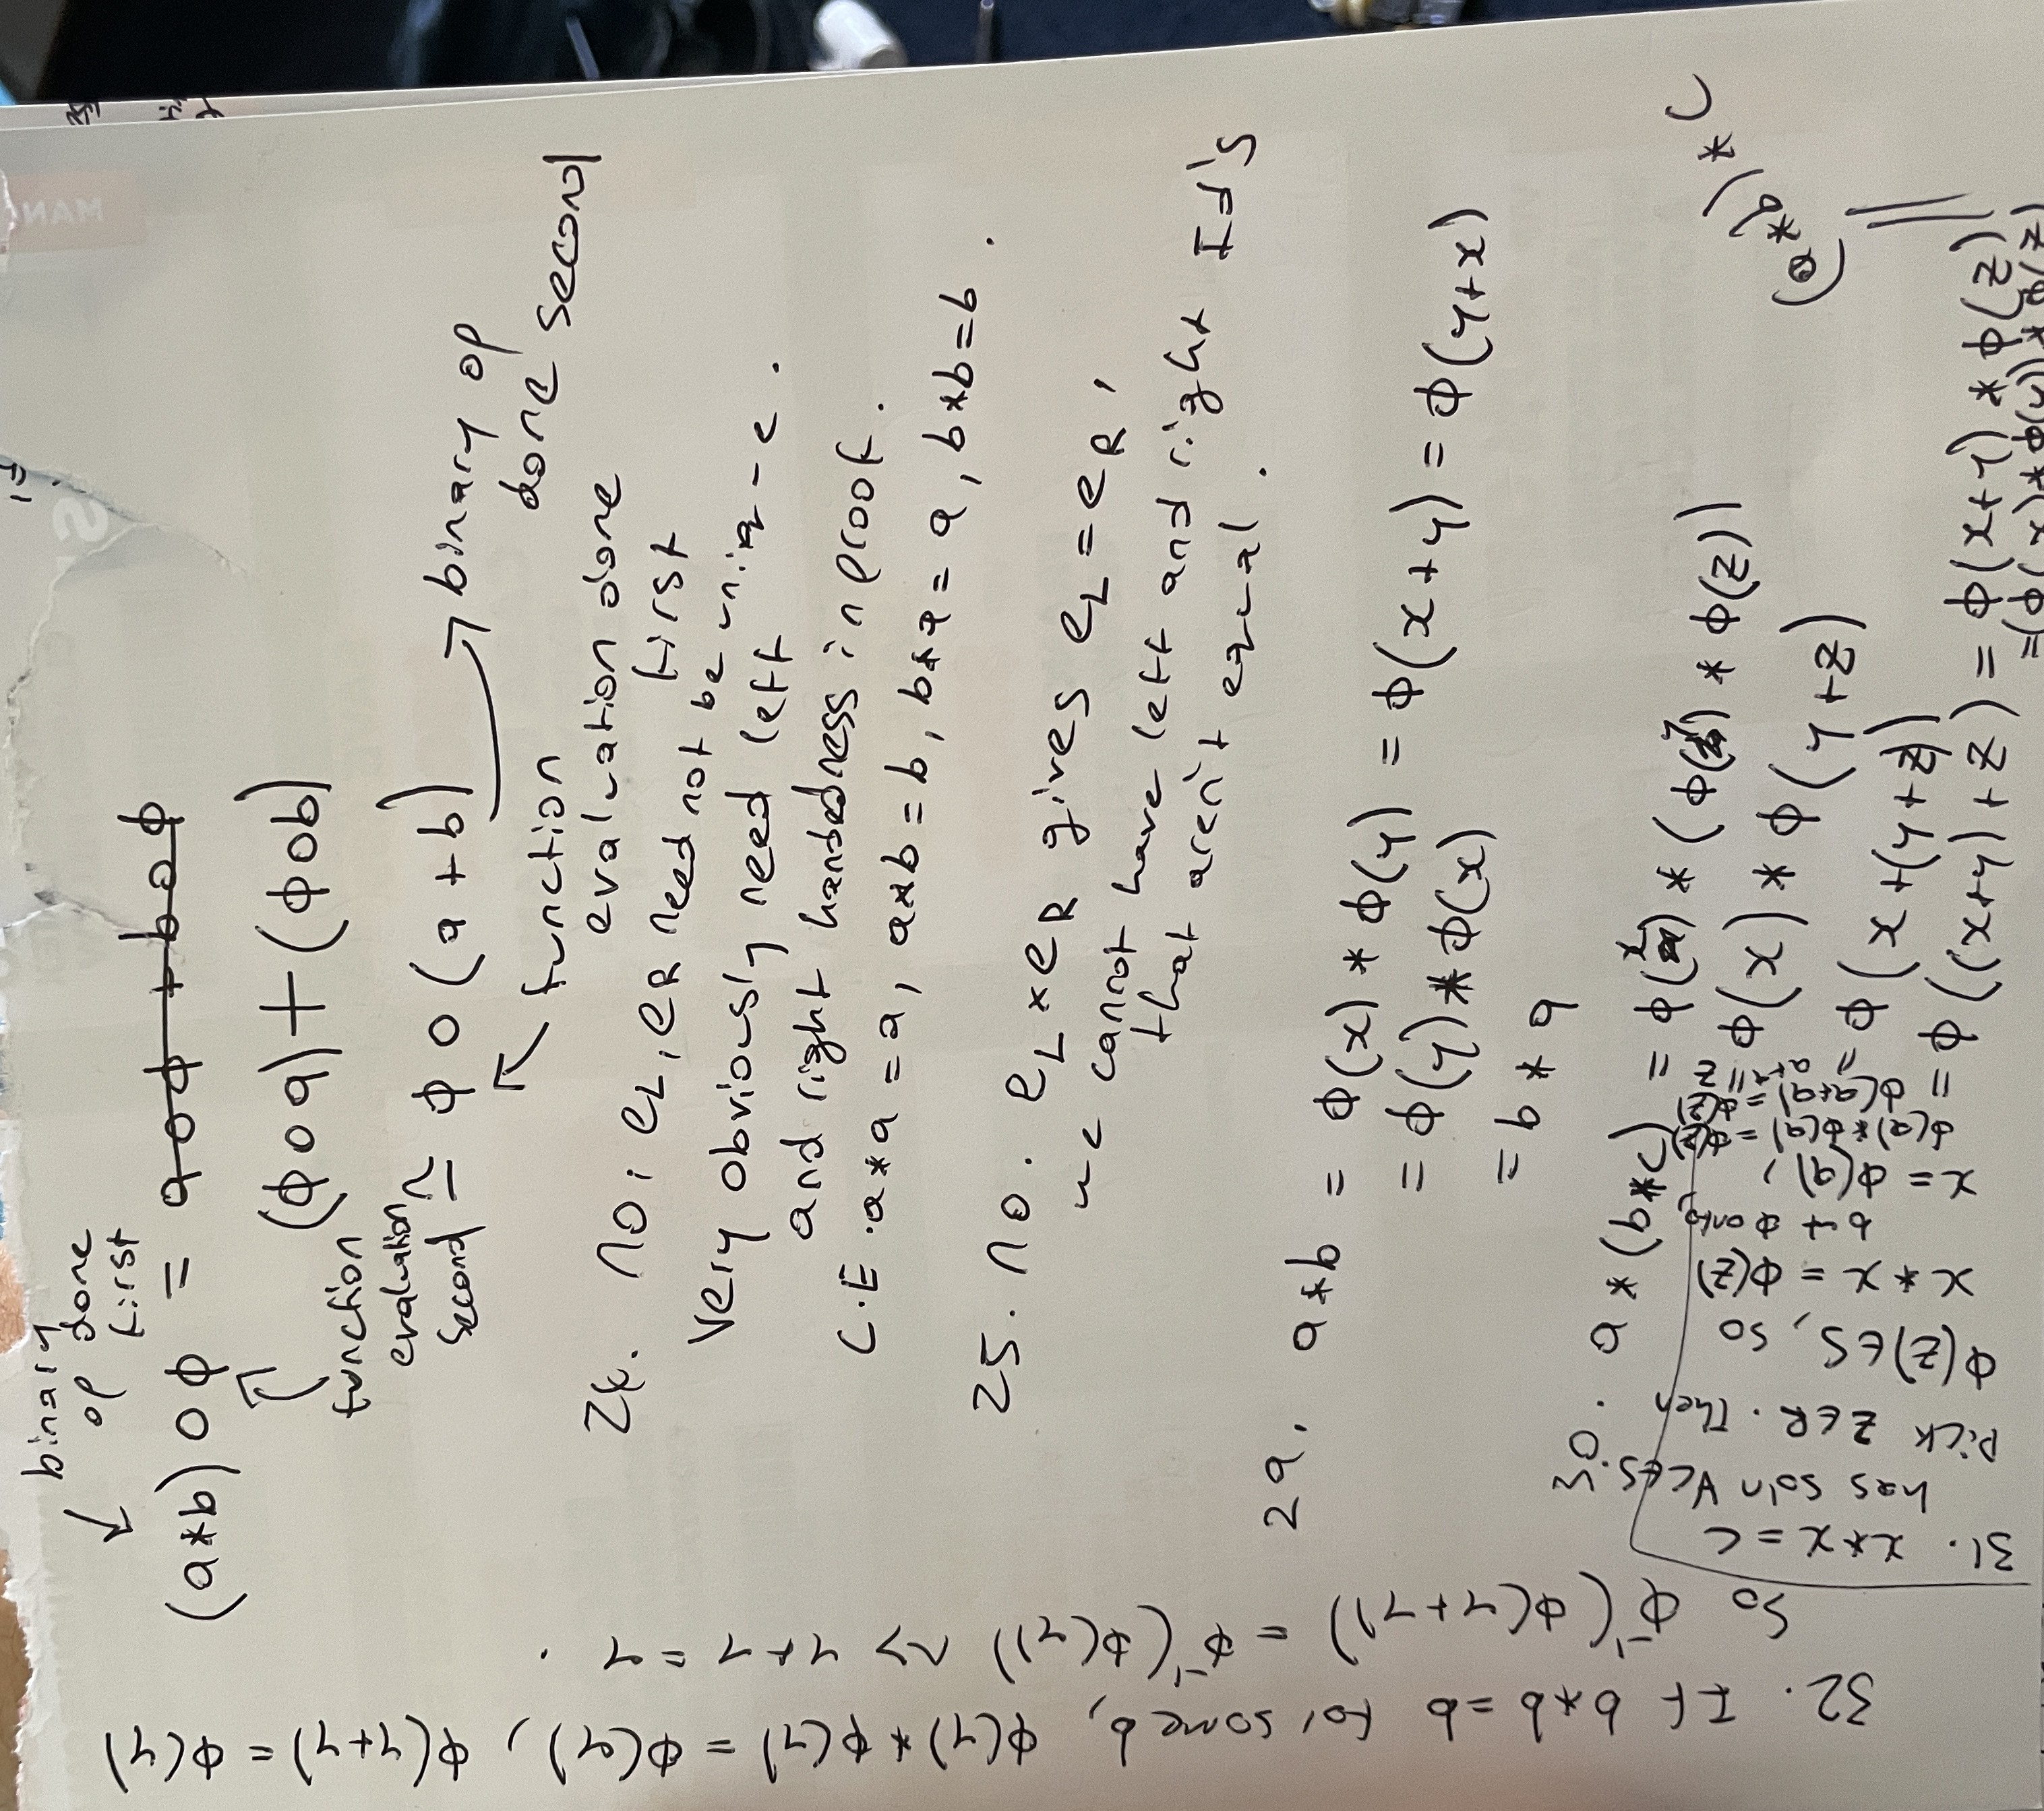
\includegraphics[scale=0.1, angle=-90]{fig/IMG_7271.jpeg}
\end{center}
\begin{center}
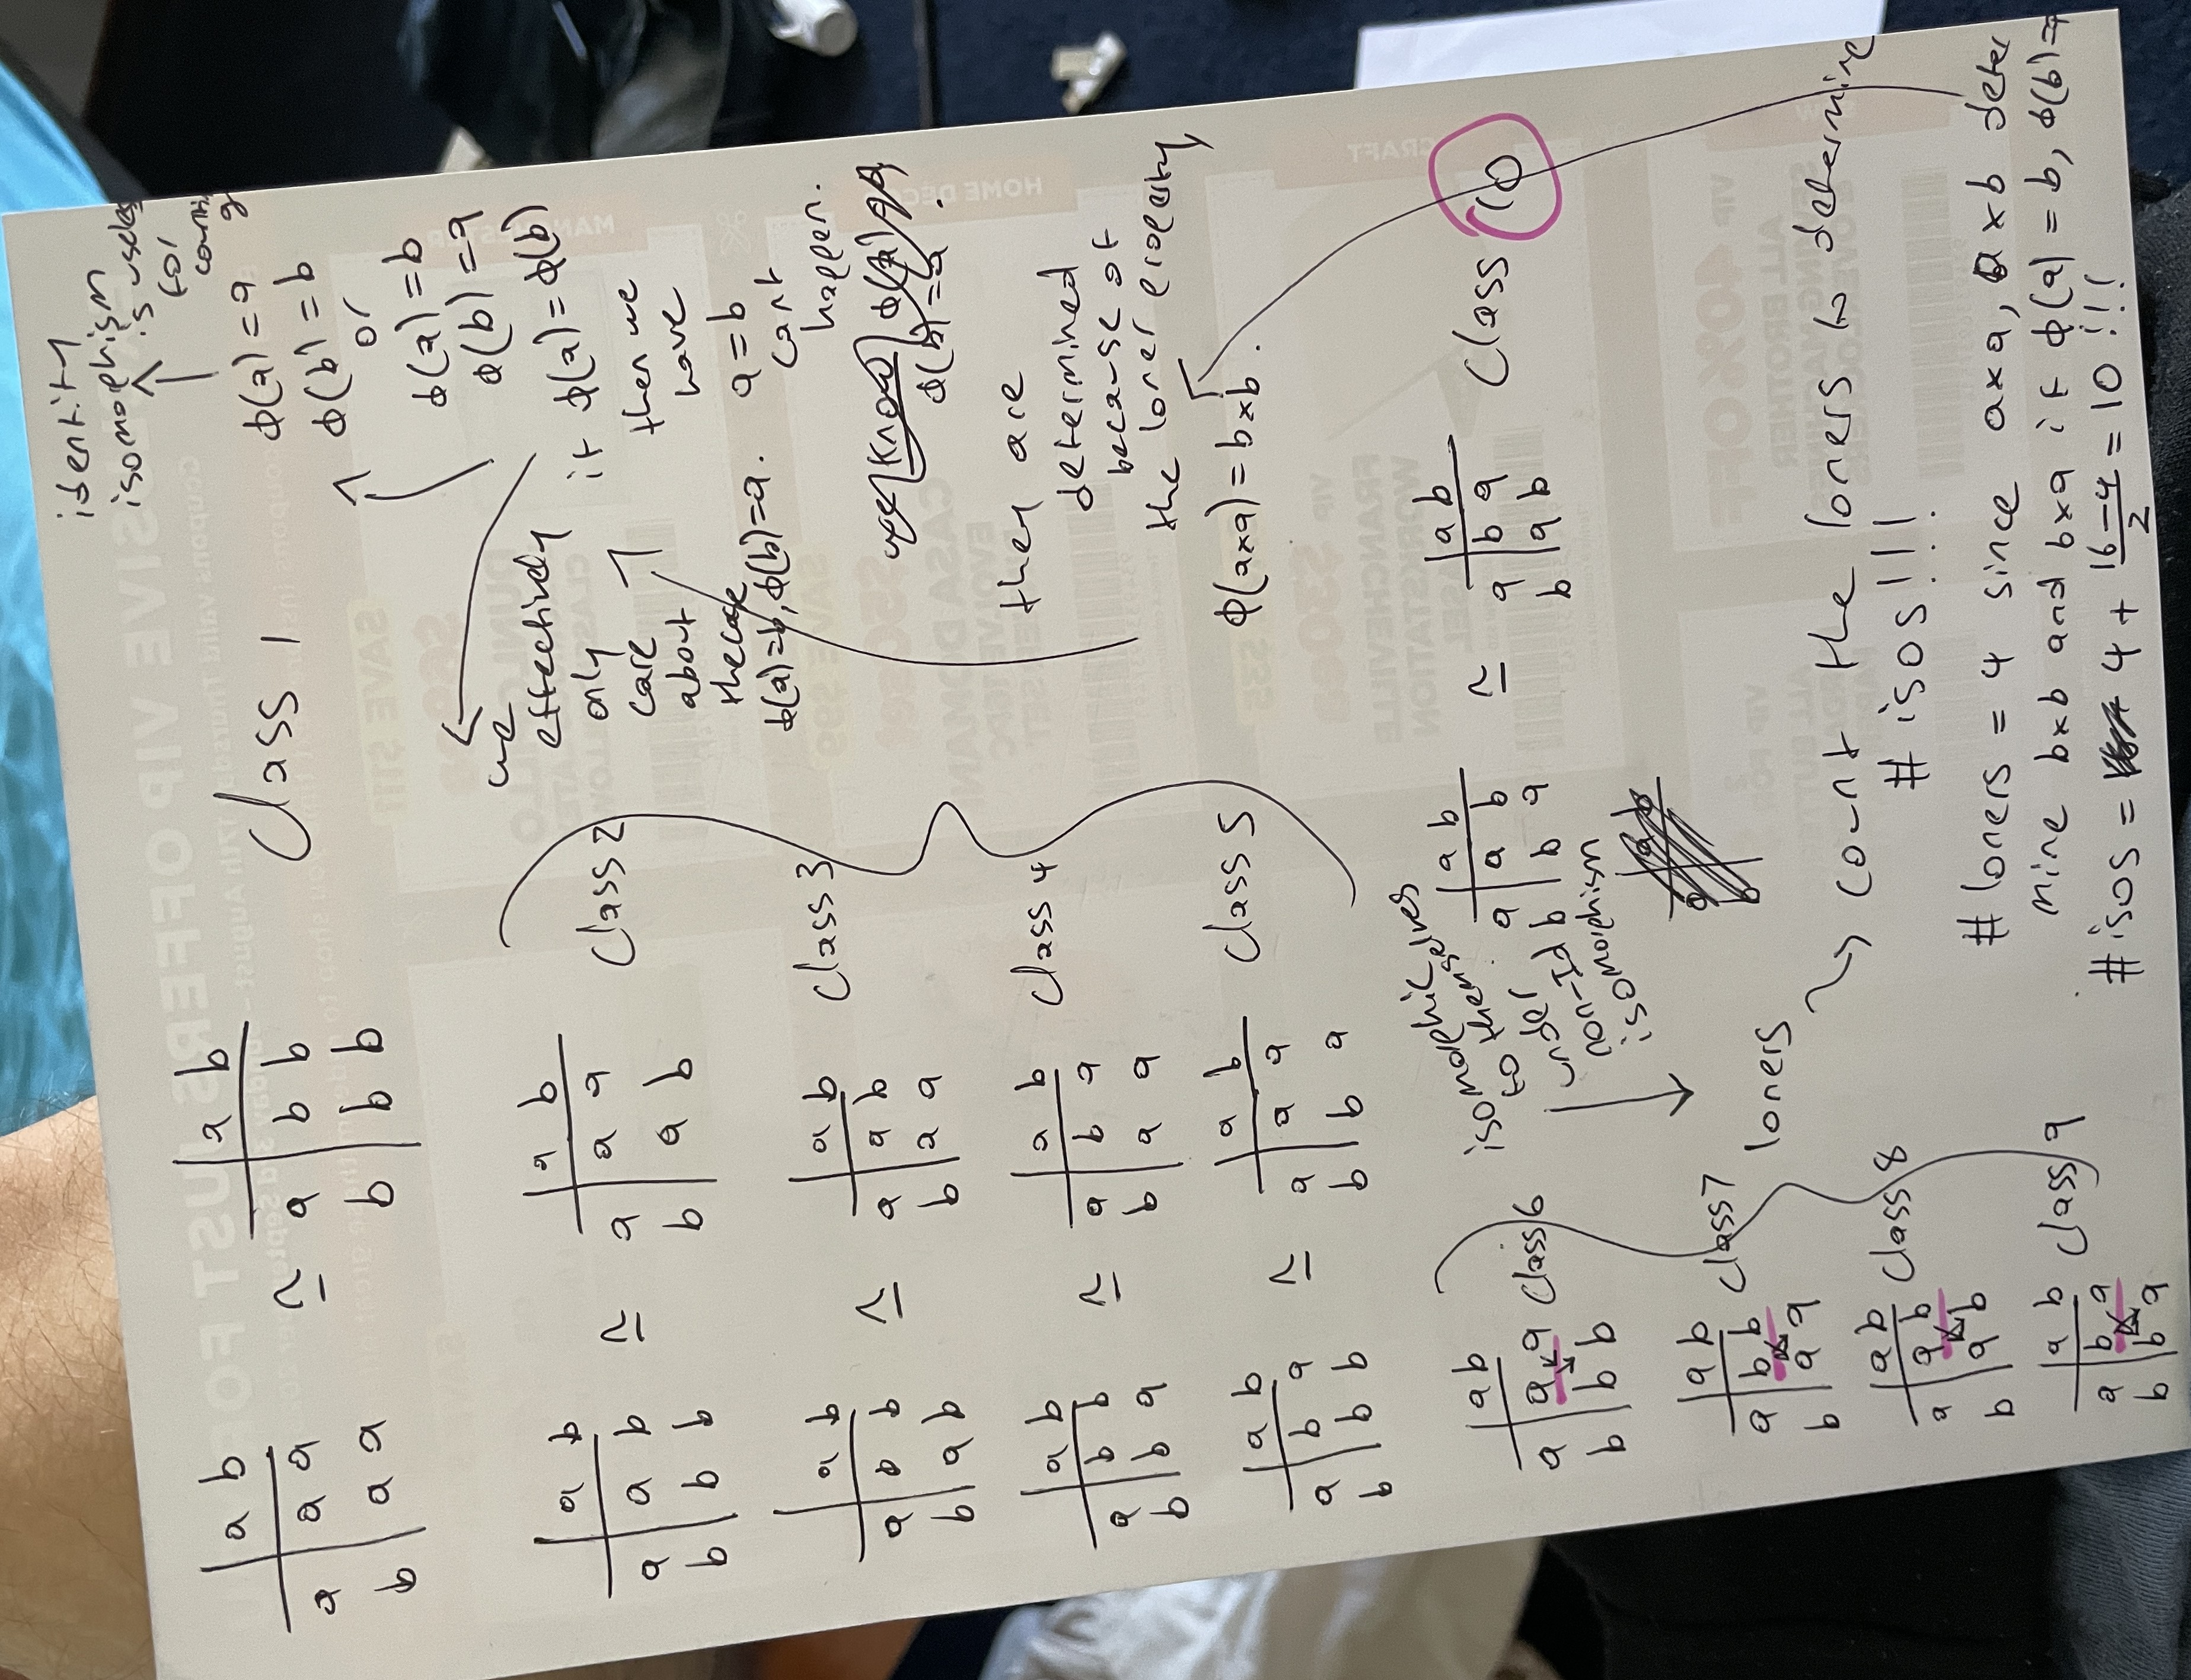
\includegraphics[scale=0.1, angle=-90]{fig/IMG_7272.jpeg}
\end{center}
\section*{Groups}
Here are some:
$$
(U, *) \text{ with } U = \{ z \in \C: |z| = 1 \}, \quad \text{$(U_n,*)$ with } U_n = \{ z \in \C: z^n = 1\}
$$
The invertible $n$ by $n$ matrices and the invertible linear maps on $\R^n$:
$$
\GLM \iso \GL
$$
To get an isomorphism, map an invertible linear function $T: \R^n \to \R^n$ to a matrix using its action on the standard basis.
Left inverses and identities plus associative is enough to define a group.
Identity is a right identity:
\begin{align*}
x + e_L &= e_L + (x + e_L)  \\ &= (x_{LL} + x_L) + (x + (x_L+x)) \\ &= x_{LL} + (x_L+x) + (x_L+x) \\ &=
x_{LL} + e_L + (x_L+x) \\ &= (x_{LL}+x_L)+x \\ &= e_L + x \\ &= x.
\end{align*}
Left inverses are right inverses also,
$$
x + x_L = e_L + x+ x_L = (x_{LL}+x_L) + x + x_L = x_{LL}+e_L+x_L = x_{LL} + x_L = e_L.
$$
\begin{center}
\includegraphics[scale=0.4, angle=-90]{fig/IMG_7275.jpeg}
\end{center}
It's easy to do the same argument with $\phi(e^\pi) = a > 0$.
Bit weirder for $(U,*) \not \simeq (\R^*,*), a^2 = a * a = \phi(e^\pi) * \phi(e^\pi) = \phi(e^{2\pi}) = 1$ but $0 \not \in \R^*$ and $a \neq 1$ since $\phi$ injective and $\phi(e^0) = 1$.
\begin{center}
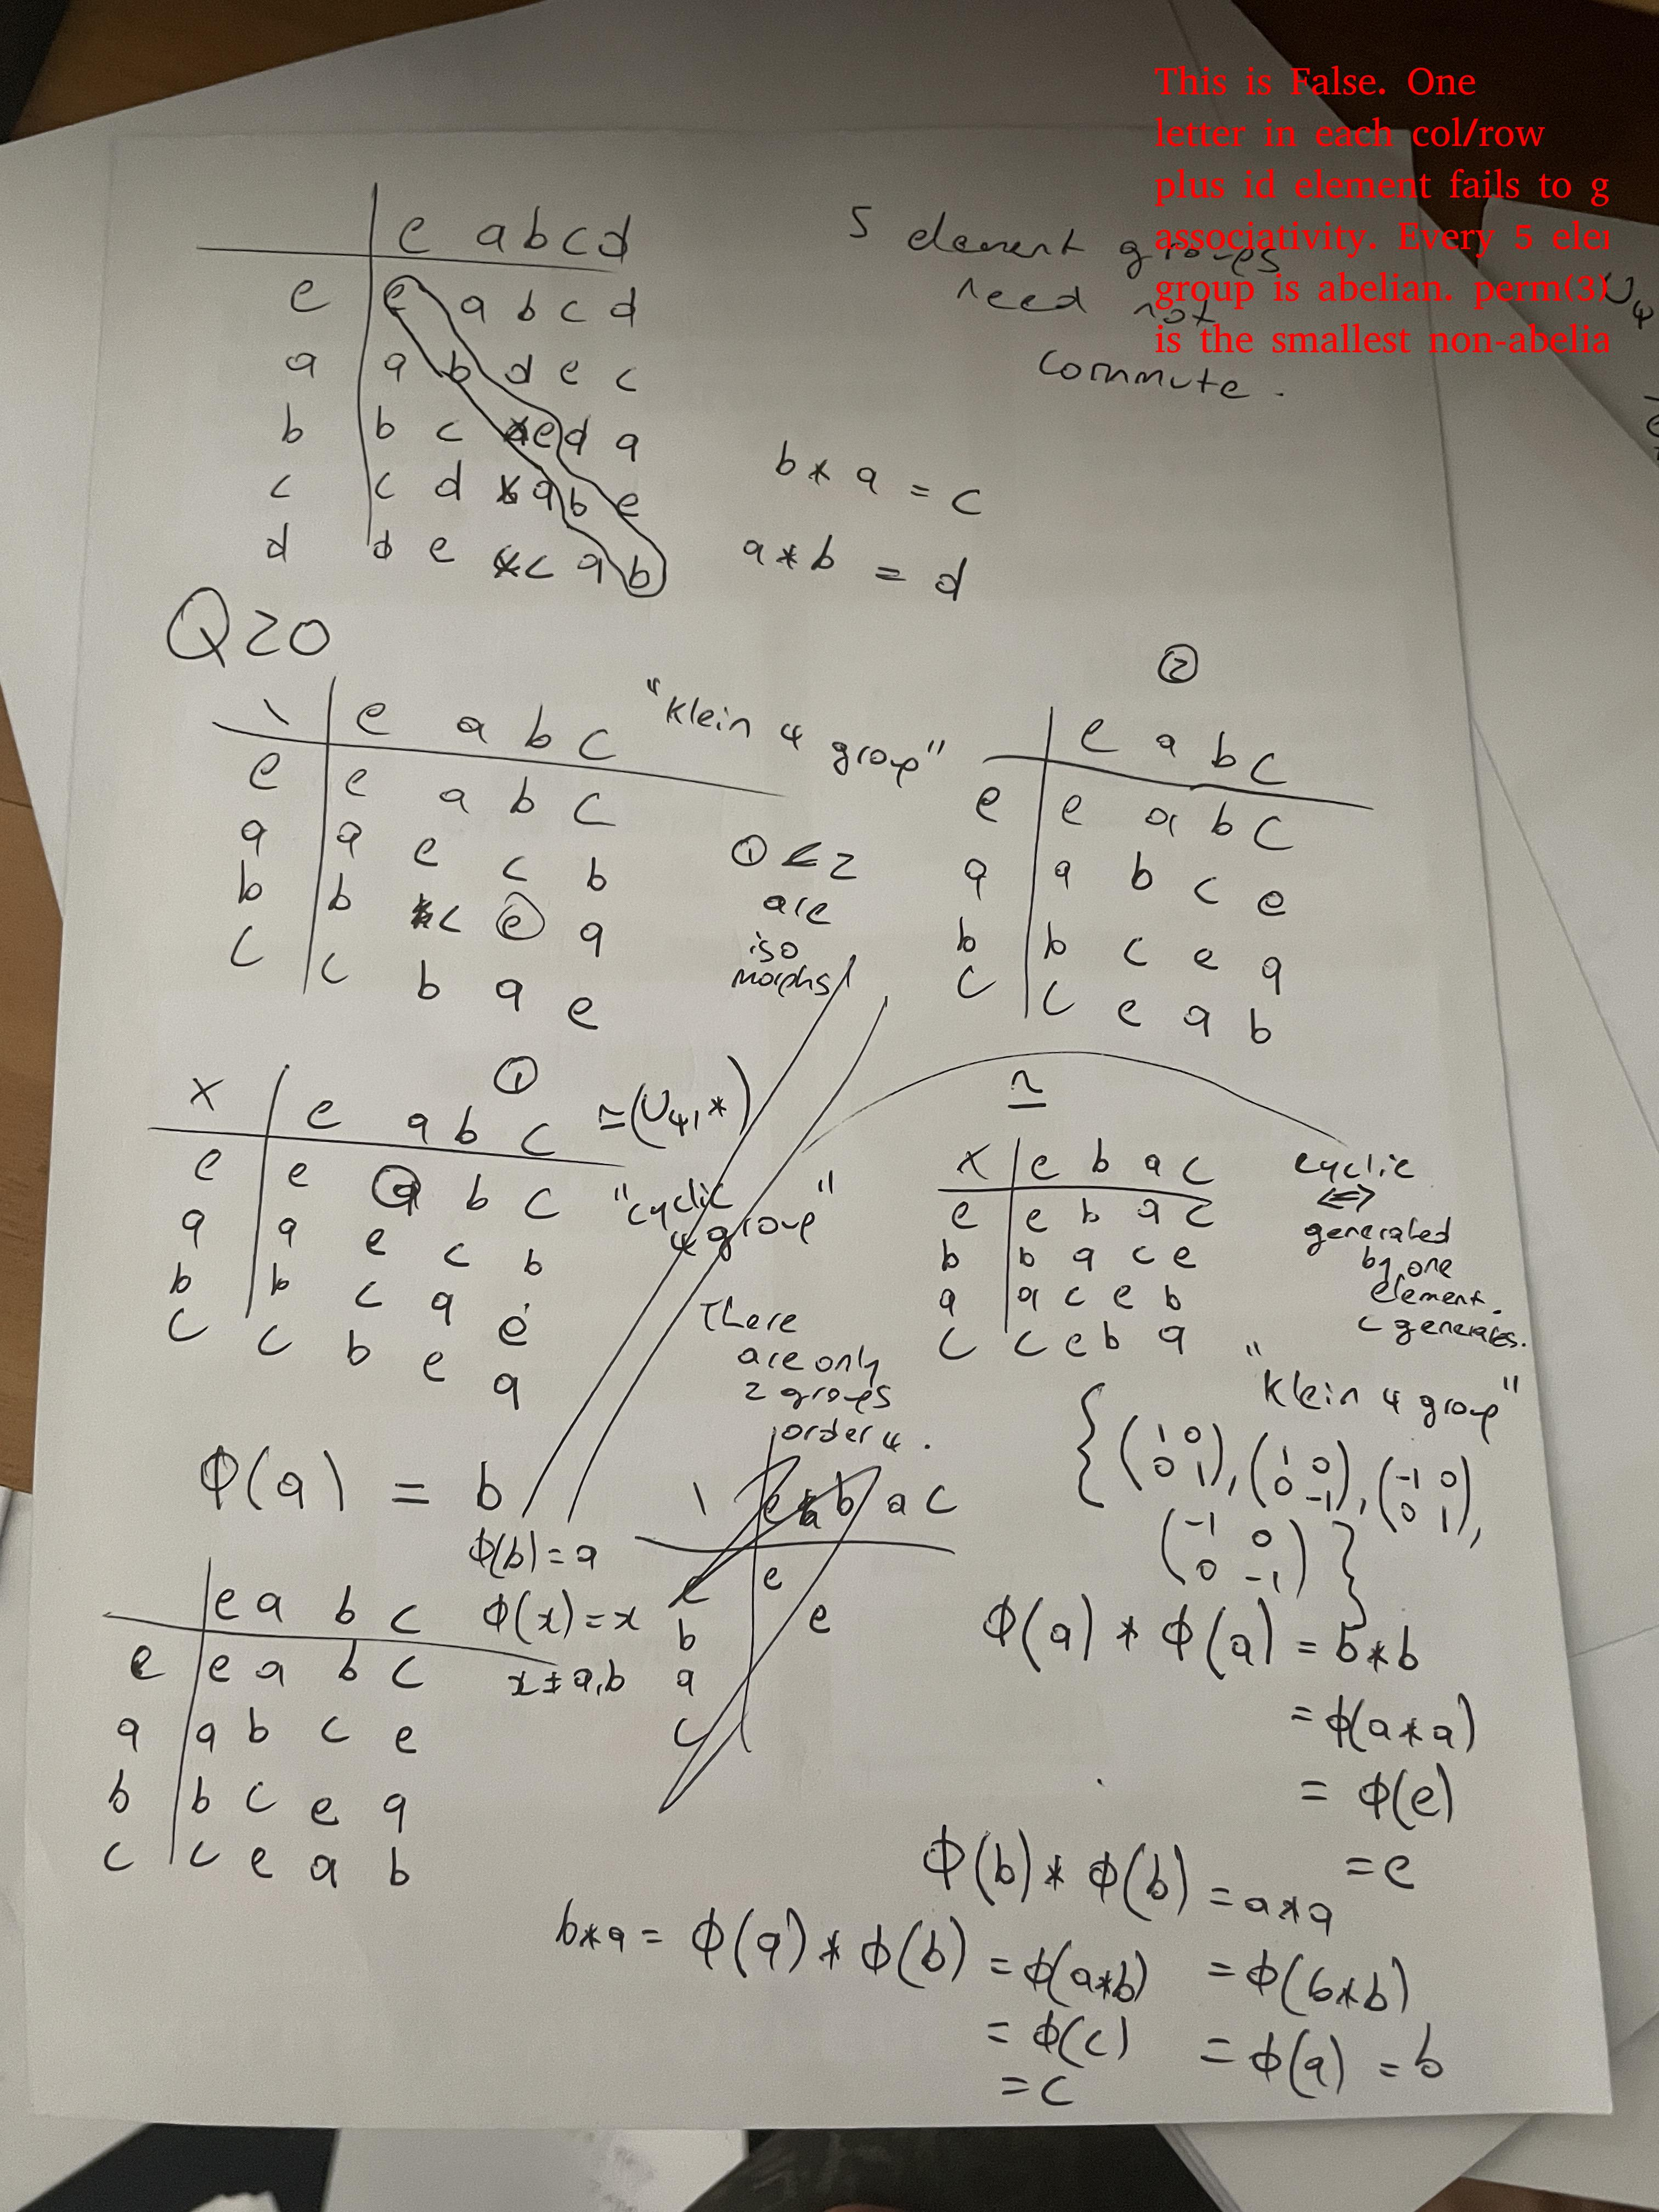
\includegraphics[scale=0.3, angle=-0]{fig/IMG_7284.jpeg}
\end{center}
\section*{Subgroups}
Subgroups are closed, contain identity and inverses. An element $a$ generates $G$ if
the cyclic subgroup $\la a \ra = \{ a^n : n \in \Z \} = G$. We say that $G$ is cyclic if there is some element that generates it.
So obviously $\la a \ra$ is a cyclic group (its always a group). Any group with no proper nontrivial subgroups is generated by every
non identity element (except the trivial group (or not, vacuous??)), so is cyclic.
\newpage{}
\section*{Cyclic Groups}
Subgroup of a cyclic group is cyclic.
\begin{center}
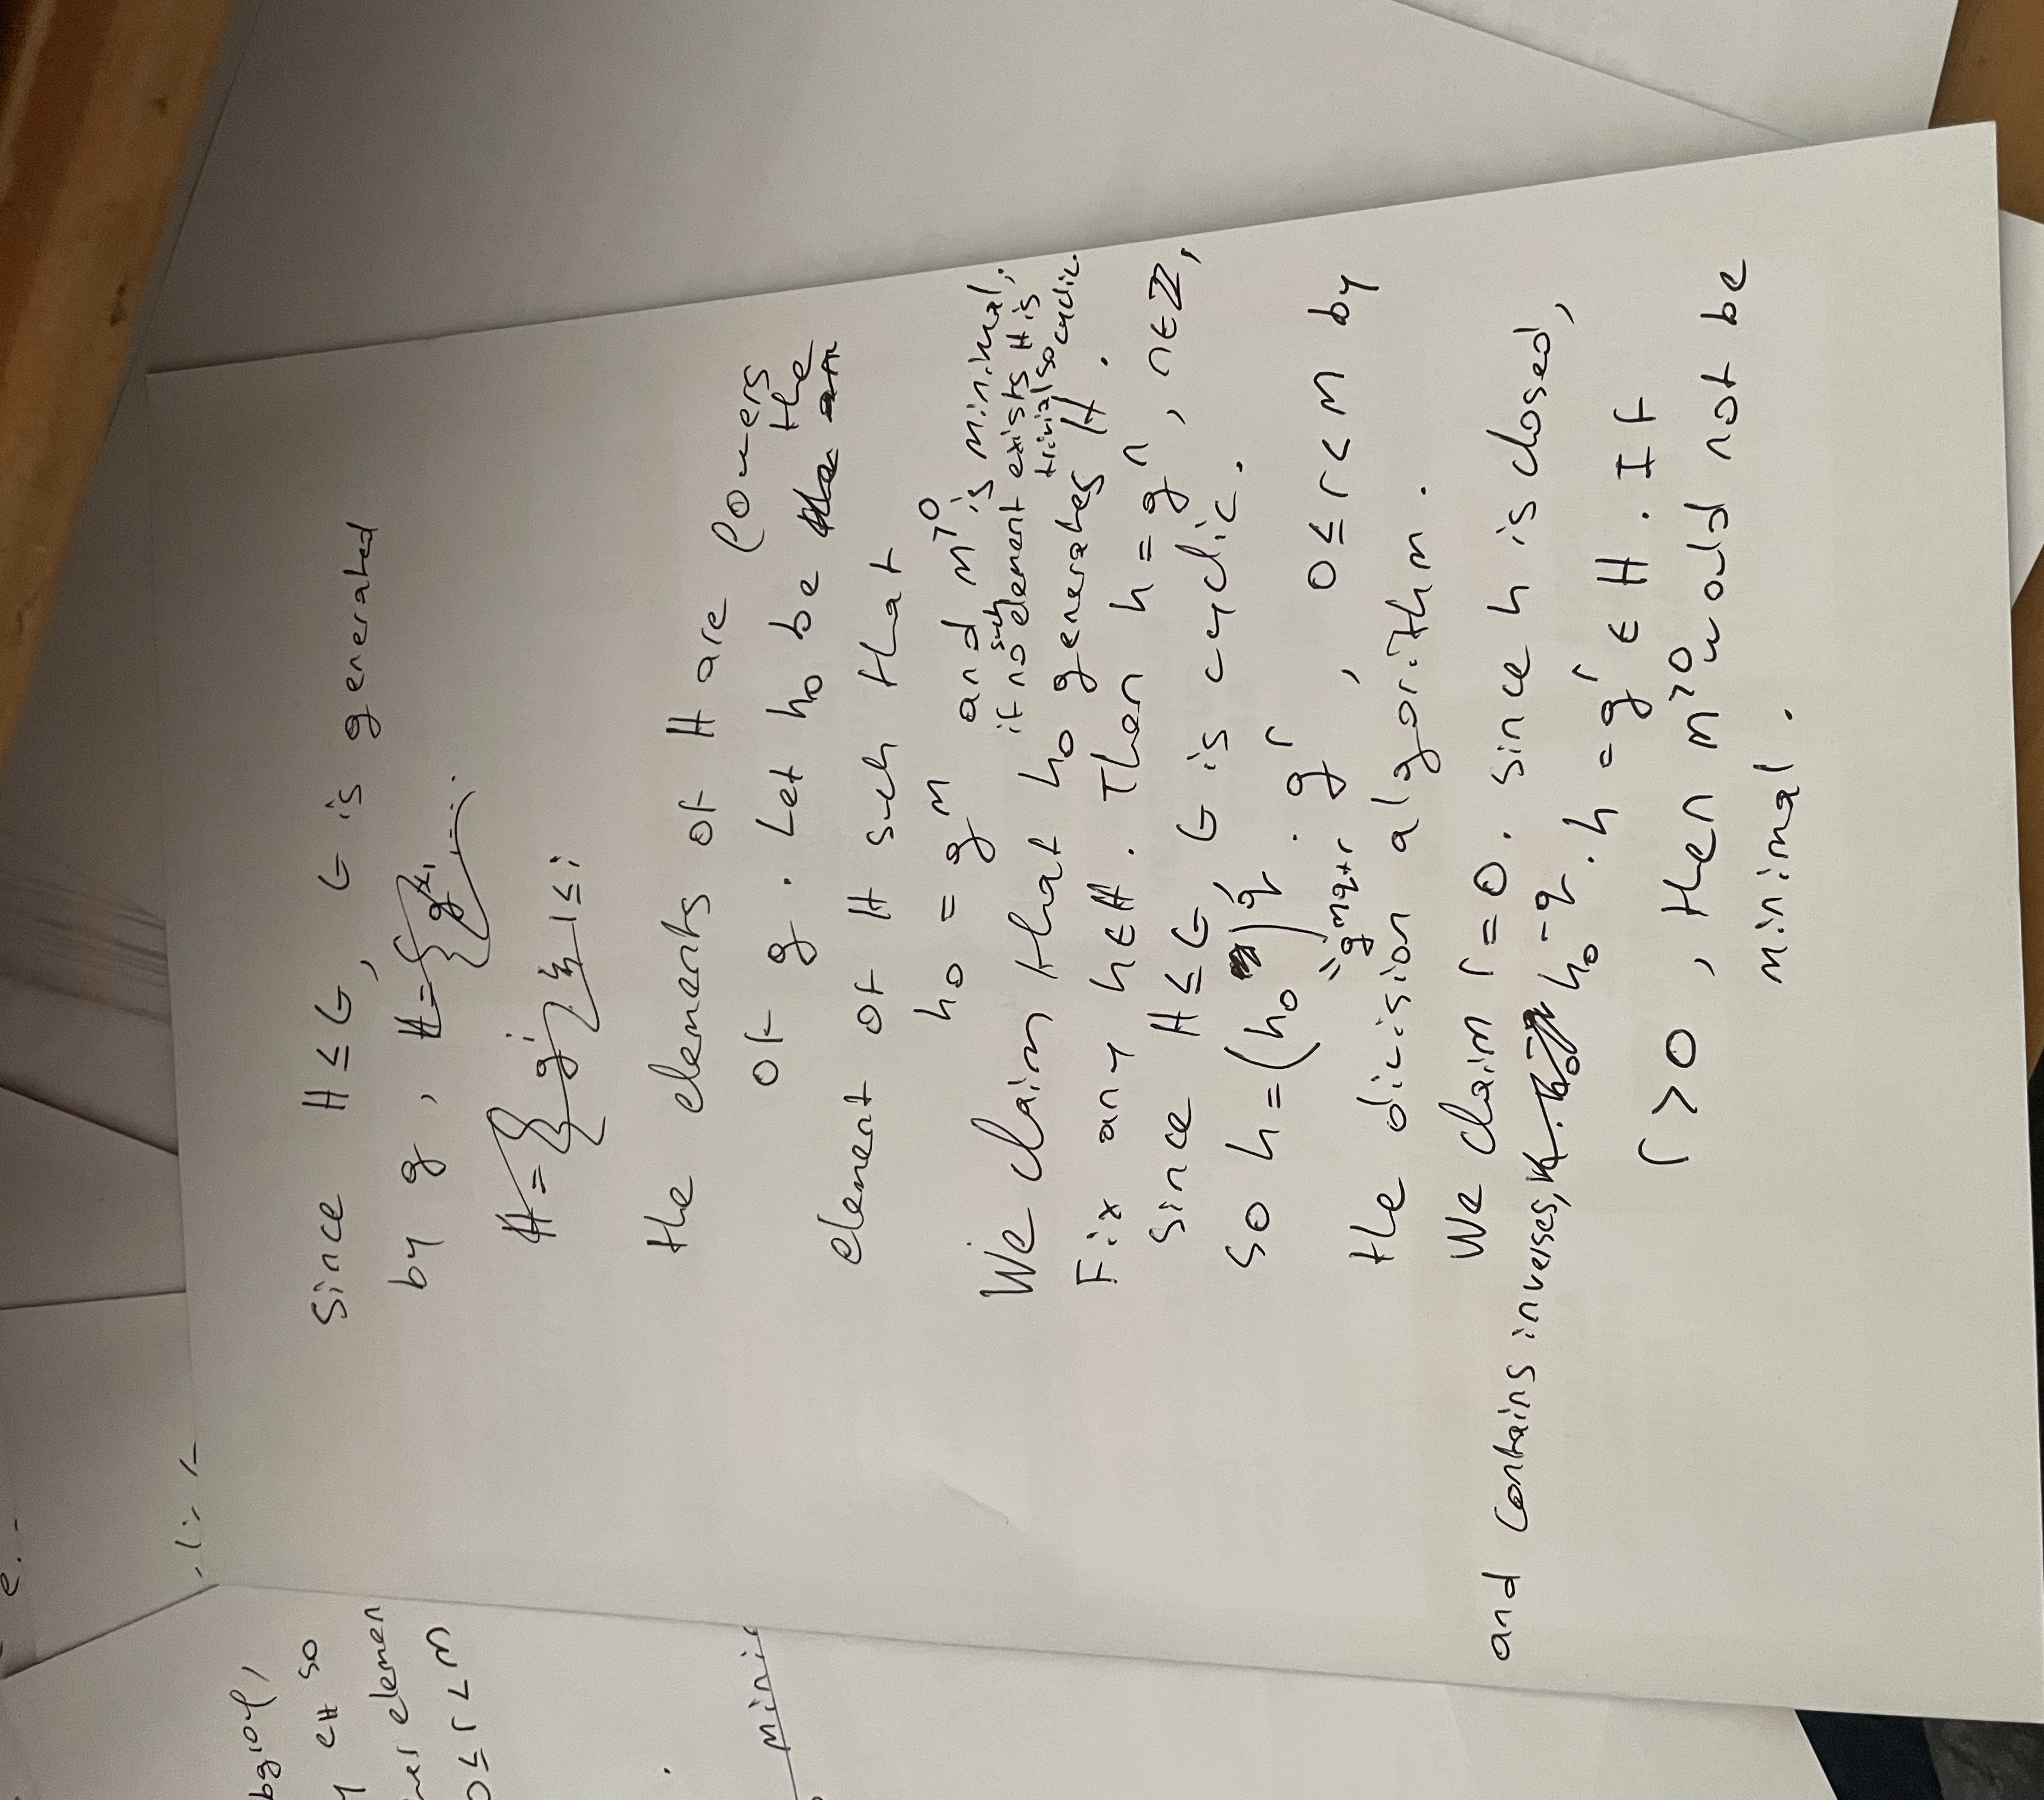
\includegraphics[scale=0.1, angle=-90]{fig/IMG_7322.jpeg}
\end{center}
Pick any subgroup $H$ of the integers under addition. Then $H$ is cyclic, so some $h$ generates $H$. So $h \in \Z$ and we must have $H = h \Z$. \\ \newline
The following is unrelated. A finicky but easy enough proof tells ya that any cyclic group is isomorphic to the integers under addition or the integers under modular addition.
The prior fact about subgroups of $\Z$ characterises subgroups of infinite cyclic groups, since their parents are isomorphic to $\Z$.
\subsection*{The hard bit: Cyclic Subgroups}
\subsubsection*{Defn}
The greatest common divisor of $m,n$ is the generator $d$ of the group $$
\{rm+sn:r,s \in \Z\}
$$
\subsubsection*{Theorem}
Let $G = \la a \ra$ be a cyclic group of order $n$. Then the order of the subgroup generated by
$a^m$ is $n \slash d$. Further, $\la a^m \ra = \la a^p \ra$ iff $\gcd(m,n) = \gcd(p,n)$.
\begin{proof}
Go read the first bit. The iff statement is badly explained. What they are saying is that
$
\{m \in \Z_n:\gcd(m,n) = d\} \subset \la d \ra
$
since $d \vert m \implies m = kd = d^k \in \la d \ra$. Any subgroup
with $n \slash d$ elements contains all elements $a^p$ of $G$ such that
$\gcd(p,n) = d$. In the case of $\Z_n$, this is just integers $p$ with $\gcd(p,n) = d$.
Then $\la a^m \ra$ contains $a^p$ and $\la a^p \ra \subset \la a^m \ra$ and similarly $\la a^m \ra \subset \la a^p \ra$ so $\la a^m \ra = \la a^p \ra$. That is to say, if the gcd's are the same then the subgroups are the same.
If the subgroups are the same, they have the same number of elements, $n \slash d_1 = n \slash d_2 \implies d_1 = d_2$.
\end{proof}
\subsubsection*{Corollary}
For each divisor $d$ of $n$, where $n$ is the order of a cyclic group $G$, there is at most one subgroup of $G$.
\subsubsection*{Corollary}
Given any generator $a$ of $G$ of order $n$, the generators are $a^p$ such that $p$ is coprime with $n$.
\subsubsection*{Defn}
The least common divisor of $m,n$ is the generator of the group $$
\{k \in \Z:m \vert k, \,\, n \vert k\}.
$$
The smallest possible LCM is $mn$ because if $k \vert m$ then $mn = (ak)n = (an)k$ so $k \vert mn$. If $m,n$ are coprime then $m \vert nk$ implies $m \vert k$. In particular,
if $n \vert k$ then $k = qn$ so $m \vert k$ implies $m \vert q$ so that $k = qn = (am)n = a(mn)$, i.e. $mn \vert k$.
\subsubsection*{Theorem}
For positive integers $m,n$
$$
\gcd(m,n) * \lcm(m,n) = mn.
$$
\begin{proof}
That $\gcd(m,n)*\lcm(m,n) \geq mn$ is easy. Since $\frac{mn}{\gcd(m,n)}$ is a multiple of both $m$ and $n$,
$\frac{mn}{\gcd(m,n)} \geq \lcm(m,n)$.
\end{proof}
\subsubsection*{Theorem}
Abelian groups with cyclic subgroups $H,K$ of coprime orders $r$ and $s$
have a cyclic subgroup of order $rs$. More generally, there is a subgroup of order $\lcm(r,s)$.
\begin{proof}
We know that $H \cap K$ is a cyclic subgroup. So it must be generated by $x = h^p  = k^q$.
Let $m = |\la x \ra|$. Then $m = r \slash \gcd(p,r) = s \slash \gcd(q,s)$
so $m \vert r$ and $m \vert s$. Then $m \vert \gcd(r,s) = 1$ and $m = 1$. So $H \cap K$ is the trivial group. Now consider the group $Z = \{xy:x \in H, y \in K  \}$ (it is a group since the whole group is Abelian).
Since $H,K$ are finite cyclic groups,  there generators $h,k$ of $H,K$.
We define
a bijection $f:\Z_r \times \Z_s \to Z$, $f(a,b) = h^a k^b$. if $f(a,b) = f(c,d)$,
then $h^{a-b} = k^{d-c} = e$ since $H \cap K  = \{e\}$. So $(a,b) = (c,d)$. Fix $z \in Z$. Then $z = xy = h^a k^b$ where $0 \leq a,b < r,s$ so $f(a,b) = z$. So $f$ is a bijection as asserted. There are $rs$ elements in $\Z_r \times \Z_s$ so the cardinality of $Z$ is $rs$.
We claim that $Z$ is cyclic when $r,s$ are coprime and $gh$ generates $Z$.
Since $r,s$ are coprime there exist integers $m_1,m_2$ so that $1 = m_1 r + m_2s$. Fix $z \in Z$ and write $z = h^ak^b$. Then we have \begin{align*}
(hk)^{bm_1r+am_2s} &= h^{bm_1r+am_2s}*k^{bm_1r+am_2s} \\ &= h^{am_2s}*k^{bm_1r} \\
&= h^{a(1-m_1r)}*k^{b(1-m_2s)} \\
&= h^a*k^b \\ &= z.
\end{align*}
N.B. The Chinese remainder theorem applies here.
\end{proof}
\begin{proof}
Easier proof. Consider $\la hk \ra$. This group is cyclic since it is generated by $hk$.
The order is no more than $rs$, since $(hk)^{rs} = e^s*e^r = e$. Suppose $p < rs$ was the order of $\la hk \ra$.
Then $h^p = k^{-p}$ so that $h^p \in H \cap K$. So $|\la h^p \ra| = d \vert r,s$ which implies $d = 1$, $\la h^p \ra = \{ e \}$. It follows that $h^p = k^p = e$, so $r,s \vert p$ (because they are the orders of $H,K$).
Then $p = ar$, so $s \vert a$ and $p = brs$, $rs \vert p$ which gives a contradiction, $p \geq rs$.
\end{proof}
\subsubsection*{Lemma for General Statement}
Given $r,s$ we can construct coprime $a,b$ so that $a \vert r$, $b \vert s$ and
$ab = \lcm(r,s)$.
\begin{proof}
Write $\lcm(r,s) = d*\frac{r}{d}*\frac{s}{d}$ and $$
d = {p_1}^{a_1} \hdots {p_n}^{a_n} * {q_1}^{b_1} \hdots {q_m}^{b_m}
$$
where $p_i \not \vert r \slash d$ and $q_i \vert r \slash d$.
Then $q_i \not \vert s \slash d$. Consider $$
a = {p_1}^{a_1} \hdots {p_n}^{a_n} * r \slash d,
\quad b = {q_1}^{b_1} \hdots {q_m}^{b_m} * s \slash d.$$
N.B.
if $ab \vert m$ then $a \vert m$,
$b \vert m$ contrapositive is if neither divide $m$ then their product doesn't.
\end{proof}
\subsubsection*{Proof for General Statement}
By the lemma, we can construct coprime divisors $a,b$ of $r,s$
with $ab = \lcm(r,s)$ so that for $r = a\del_1$, $s = b \del_2$
and $\la h^{\del_1} \ra \leq \la h \ra$, $\an{k^{\del_2}} \leq \an{k}$
we have $$|\an{h^{\del_1}}| = r \slash \gcd(\del_1,r) = r \slash \del_1 = a, \quad
|\an{k^{\del_2}}| = s \slash \gcd(\del_2,s) = s \slash \del_2 = b.$$
\subsubsection*{Example}
There is a generator of $\Z_{36}$ because it has
subgroups $\an{2}$,
$\an{3}$ with $12$ and $18$ elements. We write $12 = 6 * 2$ and $18 = 6 * 3$, then separate factors to get $6 = 3 * 2$,
$a = 2 * 12 \slash 6 = 4$, $b = 3 * 18 \slash 6 = 9$ so that $12 = 4 * 3$ and $18 = 9 * 2$.  We take these new factors $3,2$ and raise existing generators to them.
We then have $\an{3^3} = \an{9}$ of order $4$ and $\an{2^2} = \an{4}$ of order 9.
So we can generate $\Z_{36}$ with $9+4 = 13$.
\subsection*{Cayleigh Digraphs}
A group has a correspondence with a digraph with the following properties:
\begin{center}
If ya start at some point and get to some other point in two ways then the two ways will lead to the same destination from any point \\
.\\
Theres one of each generator arc to and from each point. \\
. \\
Some utter nonsense about only one arc going from a to b. \\
. \\
There exists an arc from a to b.
\end{center}
When a generator is an involution we use undirected graph edges.
An obvious implication of this is that in a group, if $a,b,\hdots,x,y$ are involutions then
$(ab \hdots xy)^{-1} = y^{-1}x^{-1} \hdots b^{-1}a^{-1} = yx \hdots ba$.
Pick a vertex $V$. If all pairs of arcs from $V$ go to the same vertex regardless of the order they are chosen then the group is commutative.
\section{Orbits, Lagrange all that Jazz}
\subsection{Perm Groups}
A permutation is a bijection of a set with itself.
If $A,B$ are finite sets of the same order, there is a bijection $f$ and the permutation groups $S_A$ and $S_B$ are isomorphic. The isomorphism is $
\phi \circ \sigma = f \circ \sigma \circ f^{-1}$. Its a homo because
$\phi \circ (\sigma \circ \tau) = f \circ (\sigma \red{\circ} \tau) \circ f^{-1} = f \circ \sigma \red{\circ (f^{-1} \circ f) \circ} \tau \circ f^{-1} = (\phi \circ \sigma) \circ (\phi \circ \tau)$.
\subsubsection{Cayleighs Theorem}
Every group is isomorphic to a subgroup of the group of permutations on the set.
Its not hard just finicky definitions and pedantry in the one to one but only onto the image stuff. Just notice that multiplication by an element permutes the elements in a group.
This allows a well defined function (not an iso) $\phi: G \to S_G$.
The inverse of left multiplication by an element is just left multiplication by the inverse of that element. Multiplication by the identity gives the identity permutation aka the identity map. We have closure, permutations of permutations are permutations. So $\phi(G)$ is a subgroup of $S_G$. The cancellation law says $\phi$ is injective. So $G$ is isomorphic to the subgroup $\phi(G)$ of $S_G$ (weird statement but yeah). \\ \newline
N.B. When computing the order of a permutation, check more than one element... \\ \newline
N.B. Right regular representations use the inverse element not the element itself.
\subsection{Orbits, Cycles, Parity of perms, Alternating Group}
Orbits are the equivalence classes of elements of a group under a permutation. Cycles are permutations with at most one orbit with order greater than 1.
Transpositions swap two elements and fix the rest (cycles of order 2). Theorem: Permutations are composed of either an odd or an even number of these.
The alternating group is the subgroup of $A_n$ of $S_n$ made up of the even permutations. The odd permutations don't form a subgroup because the identity permutation is even.

\begin{center}
\includegraphics[scale=0.5, angle=-90]{fig/IMG_7397.jpeg}
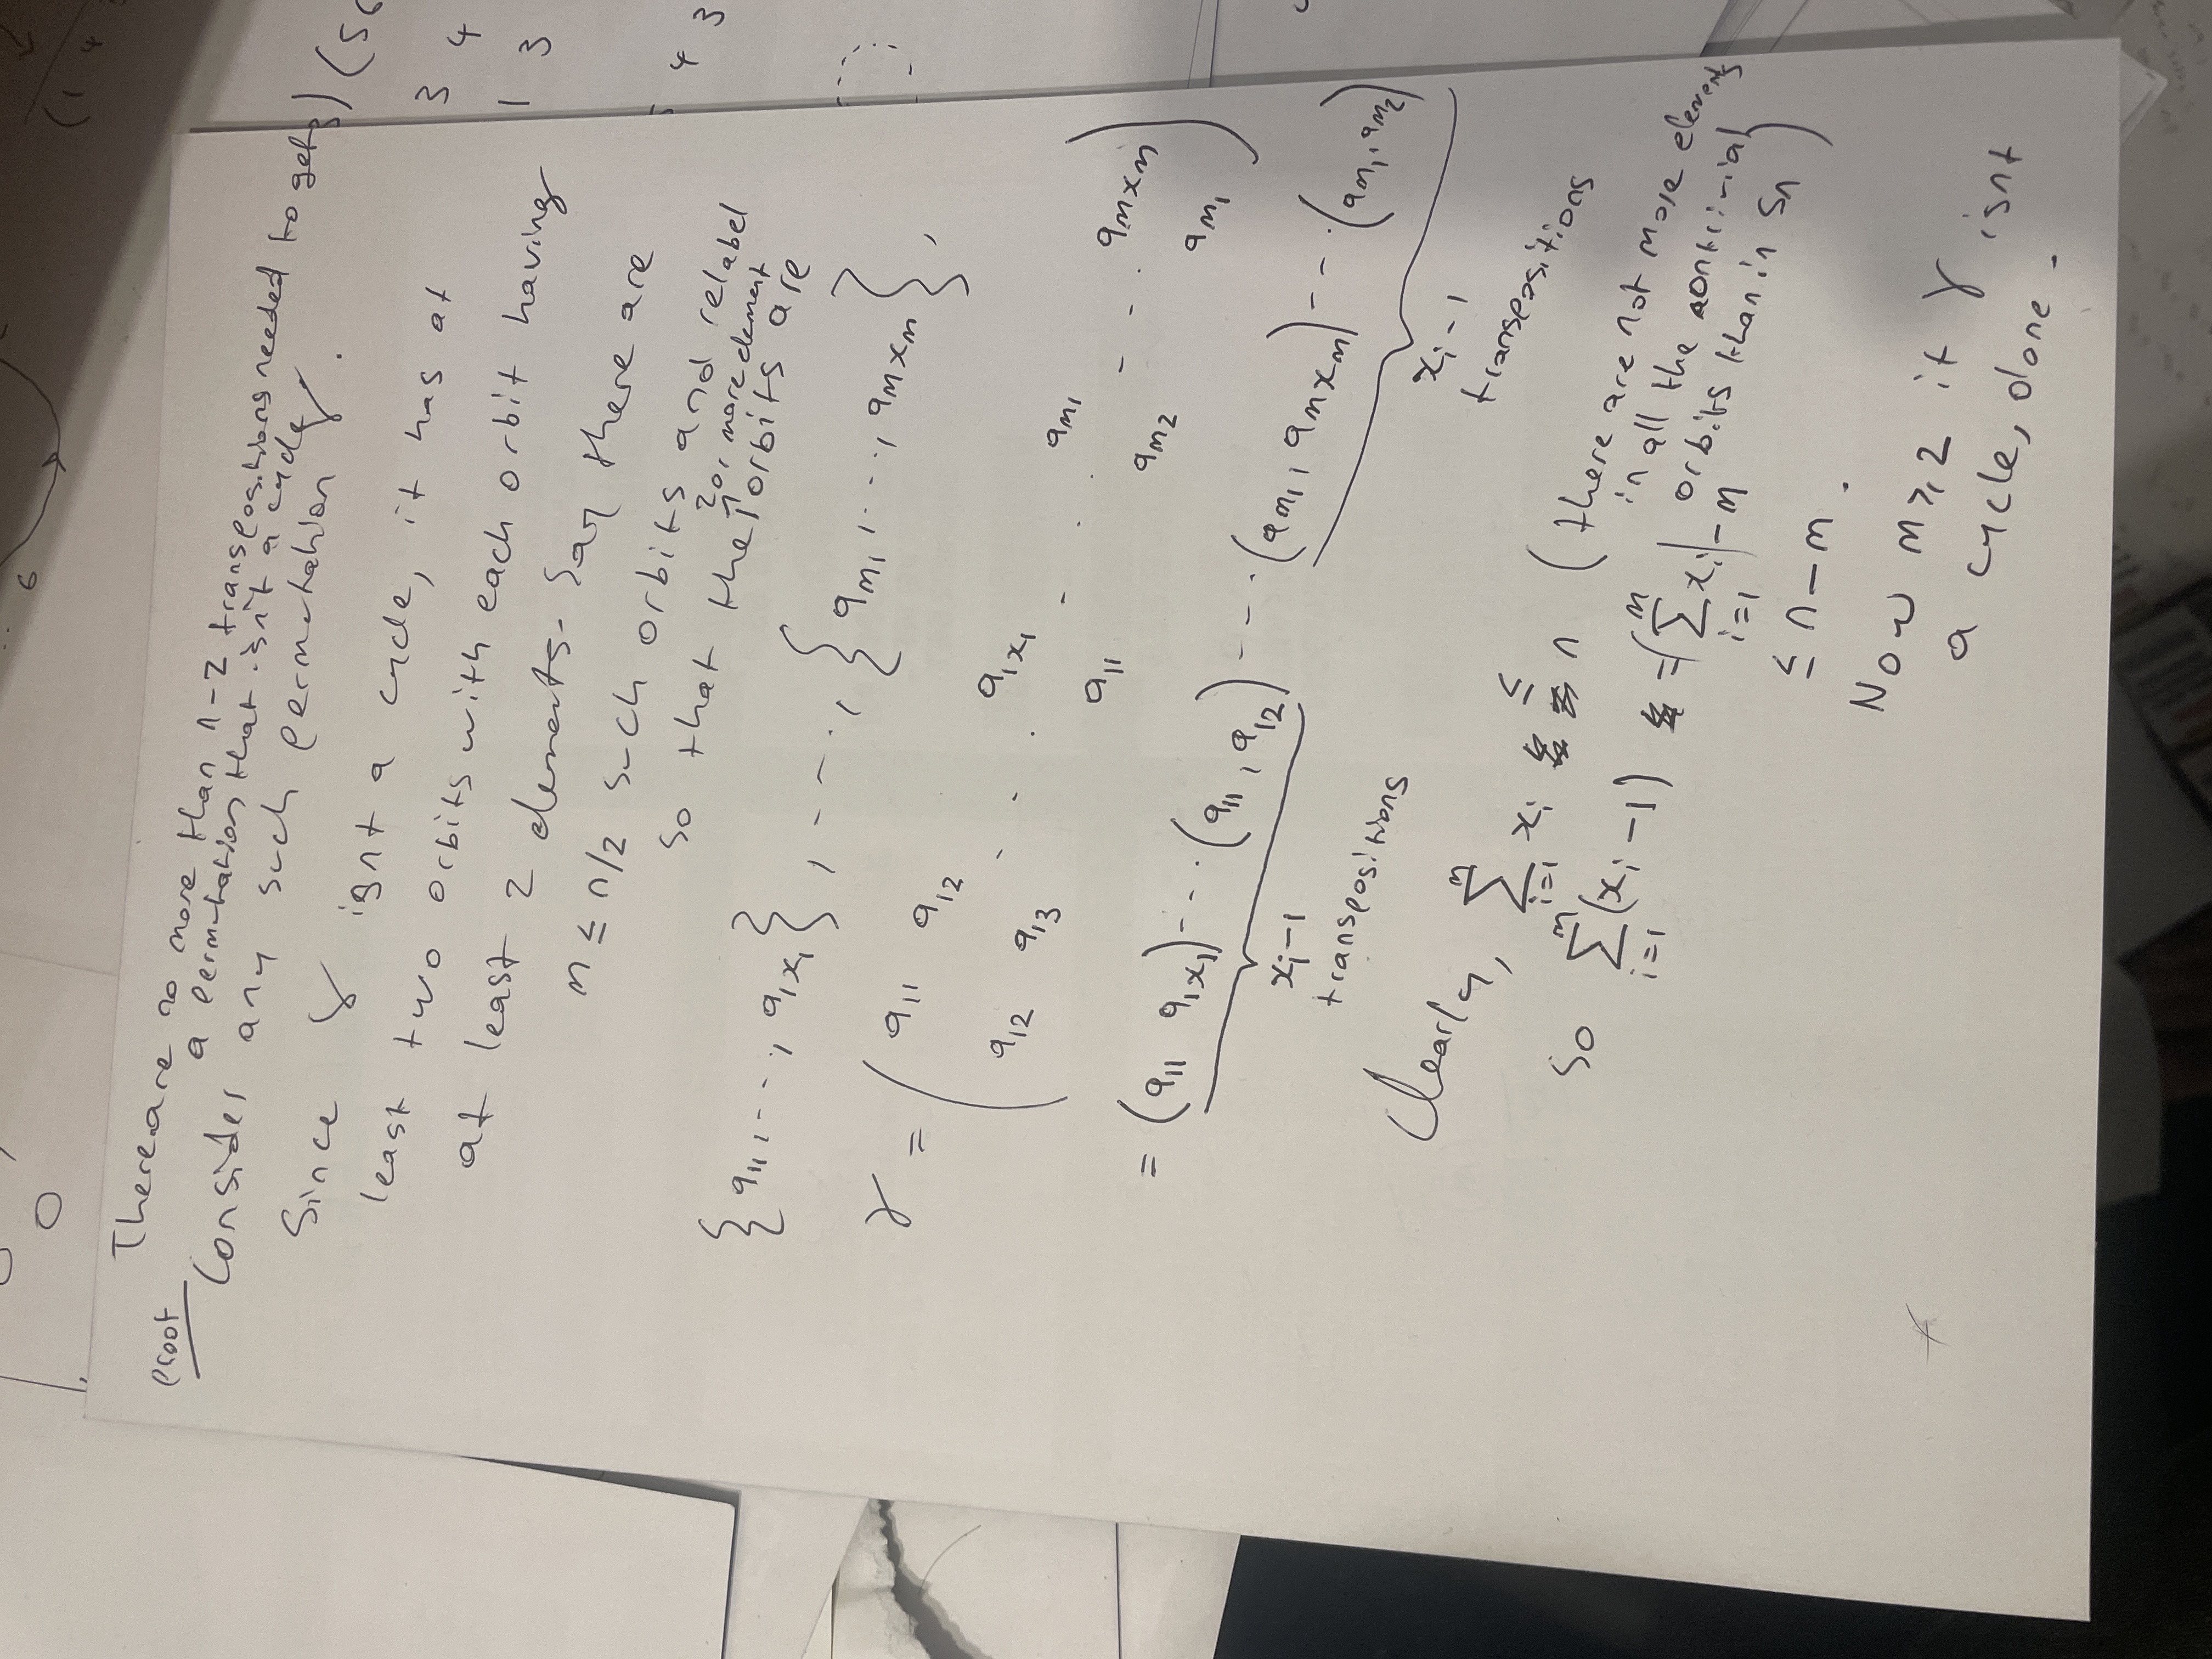
\includegraphics[scale=0.5, angle=-90]{fig/IMG_7398.jpeg}
\end{center}
\end{document}


\begin{center}
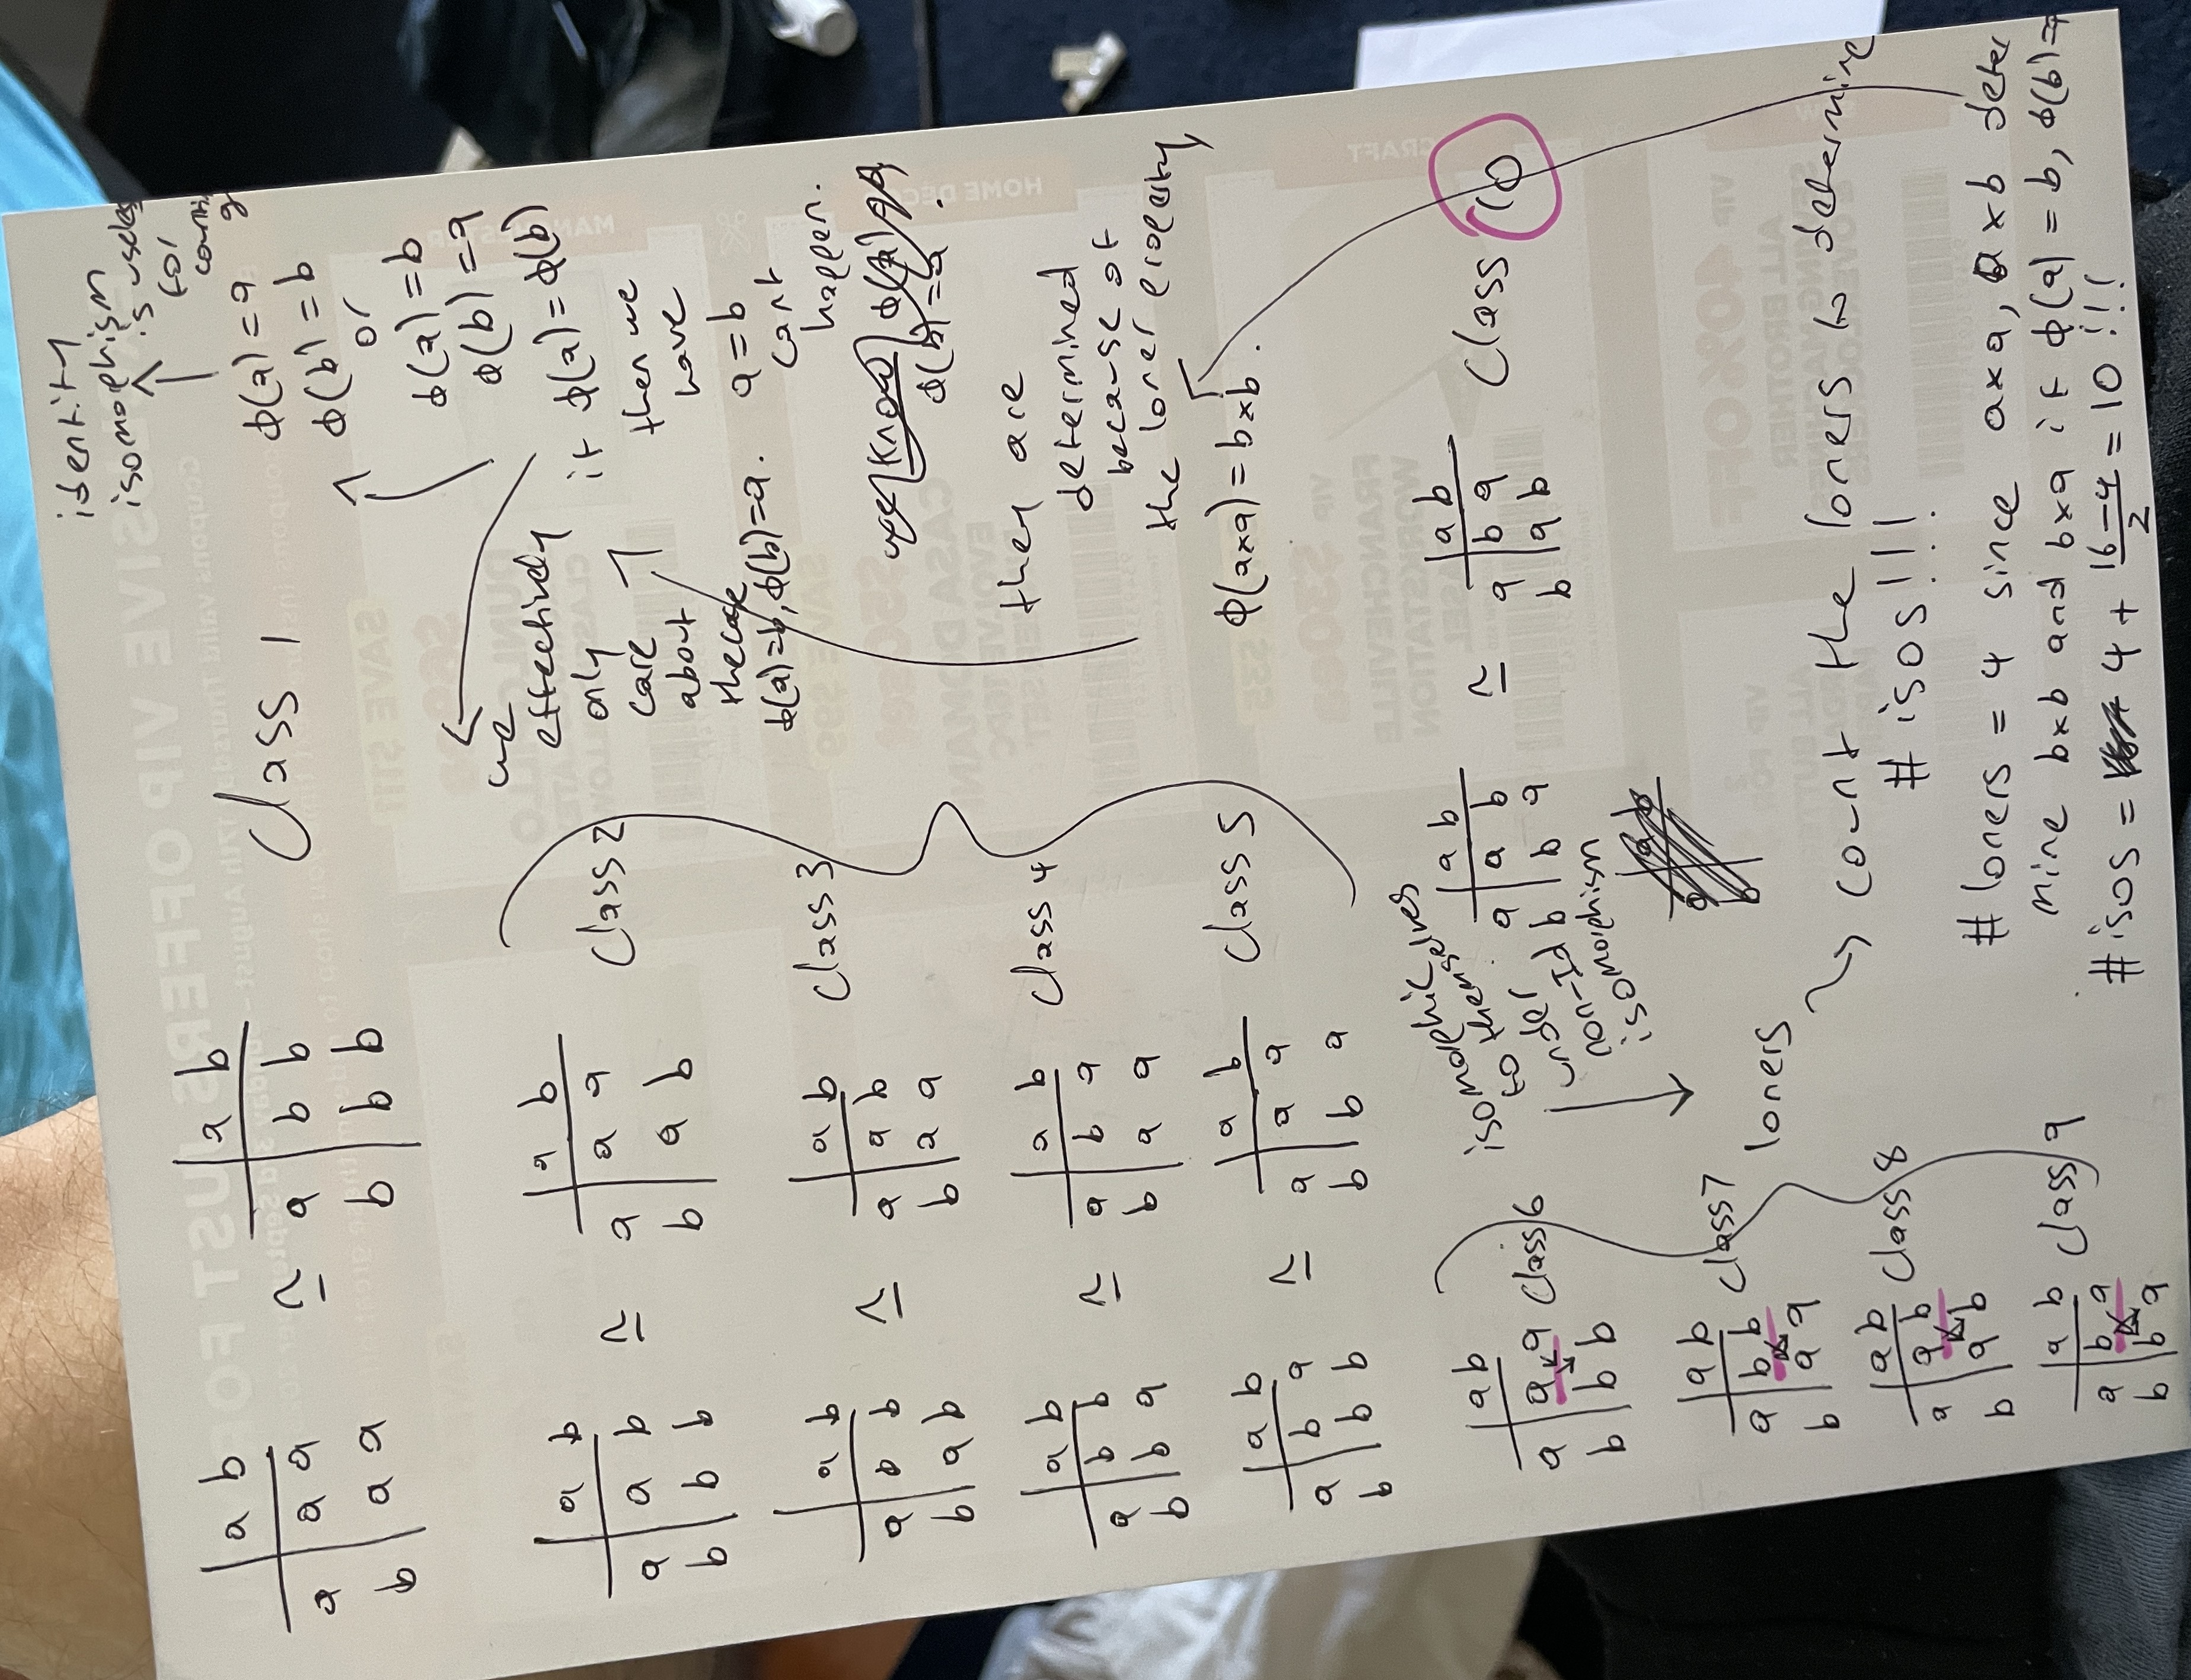
\includegraphics[scale=0.1, angle=-90]{fig/IMG_7272.jpeg}
\end{center}
